\documentclass[a4paper]{book}
\usepackage{a4wide}
\usepackage{makeidx}
\usepackage{graphicx}
\usepackage{multicol}
\usepackage{float}
\usepackage{listings}
\usepackage{color}
\usepackage{textcomp}
\usepackage{alltt}
\usepackage{times}
\usepackage{ifpdf}
\ifpdf
\usepackage[pdftex,
            pagebackref=true,
            colorlinks=true,
            linkcolor=blue,
            unicode
           ]{hyperref}
\else
\usepackage[ps2pdf,
            pagebackref=true,
            colorlinks=true,
            linkcolor=blue,
            unicode
           ]{hyperref}
\usepackage{pspicture}
\fi
\usepackage[utf8]{inputenc}
\usepackage{doxygen}
\lstset{language=C++,inputencoding=utf8,basicstyle=\footnotesize,breaklines=true,breakatwhitespace=true,tabsize=8,numbers=left }
\makeindex
\setcounter{tocdepth}{3}
\renewcommand{\footrulewidth}{0.4pt}
\begin{document}
\hypersetup{pageanchor=false}
\begin{titlepage}
\vspace*{7cm}
\begin{center}
{\Large irrBP \\[1ex]\large 0.0.1 }\\
\vspace*{1cm}
{\large Generated by Doxygen 1.7.1}\\
\vspace*{0.5cm}
{\small Thu Sep 2 2010 12:31:29}\\
\end{center}
\end{titlepage}
\clearemptydoublepage
\pagenumbering{roman}
\tableofcontents
\clearemptydoublepage
\pagenumbering{arabic}
\hypersetup{pageanchor=true}
\chapter{IrrBP 0.0.1 Documentation}
\label{index}\hypertarget{index}{}\hypertarget{index_intro}{}\section{Introduction}\label{index_intro}
Welcome to IrrBP -\/ an Irrlicht-\/Bullet Physics wrapper.

I wrote those few class to help you intagrate physics into your game, without knowing Bullet Physics Engine. The integration is very simple, and the function are very (irrlicht)user-\/friendly. You don't need to worry about optimization and memory leaks...IrrBP is alreading doing this!

IrrBP comes out without any kind of memory leak, and its fully performant.

If you have any questions or suggestions, email me at \href{mailto:stefanoguerrini93@gmail.com}{\tt stefanoguerrini93@gmail.com}\hypertarget{index_IrrBPexample}{}\section{IrrBP Integration Example}\label{index_IrrBPexample}
This example, shows you how to simply integrate bullet physics into your code. Here is it:


\begin{DoxyCode}
#include <irrlicht.h>
#include <IrrBullet.h>

using namespace irr;
using namespace core;
using namespace video;
using namespace scene;


static CIrrBPManager * bulletmgr;
static ISceneManager* smgr;
class Receiver : public IEventReceiver
{
public:
                Receiver();
                virtual bool OnEvent(const SEvent& event);
private:
};
Receiver::Receiver()
{

}

bool Receiver::OnEvent(const irr::SEvent &event)
{

        if(event.EventType == EET_MOUSE_INPUT_EVENT)
        {
                if(event.MouseInput.Event == EMIE_LMOUSE_PRESSED_DOWN)
                {
                        ISceneNode * node = smgr->addCubeSceneNode(10,0,-1,smgr->
      getActiveCamera()->getPosition());
                        CIrrBPBoxBody * body = bulletmgr->addRigidBox(node,40);
                        irr::core::vector3df rot = smgr->getActiveCamera()->getRo
      tation();
                        irr::core::matrix4 mat;
        
                        mat.setRotationDegrees(rot);
                        irr::core::vector3df forwardDir(irr::core::vector3df(mat[
      8],mat[9],mat[10]) *120);

                        body->getBodyPtr()->setLinearVelocity(irrVectorToBulletVe
      ctor(forwardDir) * 2);
        
                }
                
        }

                                
        return false;
}
int main()
{

        

        IrrlichtDevice *device =
                createDevice(video::EDT_OPENGL, core::dimension2d<u32>(640, 480))
      ;
        Receiver * recv = new Receiver();
        if (device == 0)
                return 1; // could not create selected driver.
        
        video::IVideoDriver* driver = device->getVideoDriver();
         smgr = device->getSceneManager();

        device->getFileSystem()->addZipFileArchive("map-20kdm2.pk3");

        device->setEventReceiver(recv);

        scene::IAnimatedMesh* mesh = smgr->getMesh("20kdm2.bsp");
        scene::IMeshSceneNode* node = 0;

        if (mesh)
                node = smgr->addOctreeSceneNode(mesh->getMesh(0), 0, -1, 1024);

        if (node)
                node->setPosition(core::vector3df(-1350,-130,-1400));

        
        ICameraSceneNode * cam =  smgr->addCameraSceneNodeFPS(0,100,0.1f);
        cam->setPosition(vector3df(-20,60,-30));

        
        device->getCursorControl()->setVisible(false);

        bulletmgr = createBulletManager(device);
        bulletmgr->getWorld()->setGravity(vector3df(0,-10,0));
        bulletmgr->addTrimesh(node,0);

        int xshift,yshift,zshift;
        IMeshSceneNode * Node;
        IMeshSceneNode * Node2;
        Node = smgr->addCubeSceneNode(5,0,-1,vector3df(-20,30,0));

        Node->setMaterialType(EMT_TRANSPARENT_ADD_COLOR);
        Node->setMaterialFlag(EMF_LIGHTING,false);
        Node->setMaterialTexture(0,driver->getTexture("sphere1.jpg"));
        CIrrBPBoxBody * box= bulletmgr->addRigidBox(Node,0);
        
        Node2 = smgr->addCubeSceneNode(5,0,-1,vector3df(20,0,-20));
        Node2->setMaterialType(EMT_TRANSPARENT_ADD_COLOR);
        Node2->setMaterialFlag(EMF_LIGHTING,false);
        Node2->setMaterialTexture(0,driver->getTexture("sphere1.jpg"));
        CIrrBPBoxBody * box2 = bulletmgr->addRigidBox(Node2,40);
        
        bulletmgr->buildSlideConstraint(box,box2);

        int lastFPS = -1;

        while(device->run())
        {
                if (device->isWindowActive())
                {
                        driver->beginScene(true, true, video::SColor(255,200,200,
      200));
                        bulletmgr->stepSimulation();
                        driver->setTransform(ETS_WORLD,matrix4());

                        smgr->drawAll();
                
                        int fps = driver->getFPS();

                        if (lastFPS != fps)
                        {
                                
                                core::stringw str = L"irrBP Example - HelloWorld 
      [";
                                str += driver->getName();
                                str += "] FPS:";
                                str += fps;

                                device->setWindowCaption(str.c_str());
                                lastFPS = fps;
                        }
                        driver->endScene();
                }
                else
                        device->yield();
        }

        delete recv;
        bulletmgr->drop();
        device->drop();
        return 0;
}
\end{DoxyCode}
\hypertarget{index_linker}{}\section{Linker Settings}\label{index_linker}
Before you can compile the above example, you need to include a few libraries into your project: 
\begin{DoxyEnumerate}
\item Download BulletPhysics from \href{http://code.google.com/p/bullet/downloads/list}{\tt here} 
\item Create a solution for your compiler with cmake 
\item Compile all static libraries 
\item Import 
\begin{DoxyItemize}
\item BulletCollision.lib 
\item BulletDynamics.lib 
\item BulletSoftBody.lib 
\item LinearMath.lib 
\end{DoxyItemize}
\item Add IrrBP Source and Include directory into your project 
\end{DoxyEnumerate}
\chapter{Class Index}
\section{Class Hierarchy}
This inheritance list is sorted roughly, but not completely, alphabetically:\begin{DoxyCompactList}
\item \contentsline{section}{CIrrBPAnimator}{\pageref{class_c_irr_b_p_animator}}{}
\begin{DoxyCompactList}
\item \contentsline{section}{CIrrBPCollisionDeleteAnimator}{\pageref{class_c_irr_b_p_collision_delete_animator}}{}
\item \contentsline{section}{CIrrBPDeleteAnimator}{\pageref{class_c_irr_b_p_delete_animator}}{}
\end{DoxyCompactList}
\item \contentsline{section}{CIrrBPCollisionObject}{\pageref{class_c_irr_b_p_collision_object}}{}
\begin{DoxyCompactList}
\item \contentsline{section}{CIrrBPRigidBody}{\pageref{class_c_irr_b_p_rigid_body}}{}
\begin{DoxyCompactList}
\item \contentsline{section}{CIrrBPBoxBody}{\pageref{class_c_irr_b_p_box_body}}{}
\item \contentsline{section}{CIrrBPCapsuleBody}{\pageref{class_c_irr_b_p_capsule_body}}{}
\item \contentsline{section}{CIrrBPConeBody}{\pageref{class_c_irr_b_p_cone_body}}{}
\item \contentsline{section}{CIrrBPCylinderBody}{\pageref{class_c_irr_b_p_cylinder_body}}{}
\item \contentsline{section}{CIrrBPSphereBody}{\pageref{class_c_irr_b_p_sphere_body}}{}
\item \contentsline{section}{CIrrBPTrimesh}{\pageref{class_c_irr_b_p_trimesh}}{}
\end{DoxyCompactList}
\item \contentsline{section}{CIrrBPSoftBody}{\pageref{class_c_irr_b_p_soft_body}}{}
\begin{DoxyCompactList}
\item \contentsline{section}{CIrrBPPatchSoftBody}{\pageref{class_c_irr_b_p_patch_soft_body}}{}
\item \contentsline{section}{CIrrBPRopeSoftBody}{\pageref{class_c_irr_b_p_rope_soft_body}}{}
\end{DoxyCompactList}
\end{DoxyCompactList}
\item \contentsline{section}{CIrrBPConstraint}{\pageref{class_c_irr_b_p_constraint}}{}
\begin{DoxyCompactList}
\item \contentsline{section}{CIrrBPConeTwistConstraint}{\pageref{class_c_irr_b_p_cone_twist_constraint}}{}
\item \contentsline{section}{CIrrBPHingeConstraint}{\pageref{class_c_irr_b_p_hinge_constraint}}{}
\item \contentsline{section}{CIrrBPP2PConstraint}{\pageref{class_c_irr_b_p_p2_p_constraint}}{}
\item \contentsline{section}{CIrrBPSlideConstraint}{\pageref{class_c_irr_b_p_slide_constraint}}{}
\end{DoxyCompactList}
\item \contentsline{section}{CIrrBPDebugDrawer}{\pageref{class_c_irr_b_p_debug_drawer}}{}
\item \contentsline{section}{CIrrBPManager}{\pageref{class_c_irr_b_p_manager}}{}
\item \contentsline{section}{CIrrBPWorld}{\pageref{class_c_irr_b_p_world}}{}
\item \contentsline{section}{CMotionState}{\pageref{class_c_motion_state}}{}
\end{DoxyCompactList}

\chapter{Class Index}
\section{Class List}
Here are the classes, structs, unions and interfaces with brief descriptions:\begin{DoxyCompactList}
\item\contentsline{section}{\hyperlink{class_c_irr_b_p_animator}{CIrrBPAnimator} }{\pageref{class_c_irr_b_p_animator}}{}
\item\contentsline{section}{\hyperlink{class_c_irr_b_p_box_body}{CIrrBPBoxBody} }{\pageref{class_c_irr_b_p_box_body}}{}
\item\contentsline{section}{\hyperlink{class_c_irr_b_p_capsule_body}{CIrrBPCapsuleBody} }{\pageref{class_c_irr_b_p_capsule_body}}{}
\item\contentsline{section}{\hyperlink{class_c_irr_b_p_collision_delete_animator}{CIrrBPCollisionDeleteAnimator} }{\pageref{class_c_irr_b_p_collision_delete_animator}}{}
\item\contentsline{section}{\hyperlink{class_c_irr_b_p_cone_body}{CIrrBPConeBody} }{\pageref{class_c_irr_b_p_cone_body}}{}
\item\contentsline{section}{\hyperlink{class_c_irr_b_p_cone_twist_constraint}{CIrrBPConeTwistConstraint} }{\pageref{class_c_irr_b_p_cone_twist_constraint}}{}
\item\contentsline{section}{\hyperlink{class_c_irr_b_p_constraint}{CIrrBPConstraint} }{\pageref{class_c_irr_b_p_constraint}}{}
\item\contentsline{section}{\hyperlink{class_c_irr_b_p_cylinder_body}{CIrrBPCylinderBody} }{\pageref{class_c_irr_b_p_cylinder_body}}{}
\item\contentsline{section}{\hyperlink{class_c_irr_b_p_debug_drawer}{CIrrBPDebugDrawer} (Should not be used. Only for internal use )}{\pageref{class_c_irr_b_p_debug_drawer}}{}
\item\contentsline{section}{\hyperlink{class_c_irr_b_p_delete_animator}{CIrrBPDeleteAnimator} }{\pageref{class_c_irr_b_p_delete_animator}}{}
\item\contentsline{section}{\hyperlink{class_c_irr_b_p_hinge_constraint}{CIrrBPHingeConstraint} }{\pageref{class_c_irr_b_p_hinge_constraint}}{}
\item\contentsline{section}{\hyperlink{class_c_irr_b_p_manager}{CIrrBPManager} }{\pageref{class_c_irr_b_p_manager}}{}
\item\contentsline{section}{\hyperlink{class_c_irr_b_p_p2_p_constraint}{CIrrBPP2PConstraint} }{\pageref{class_c_irr_b_p_p2_p_constraint}}{}
\item\contentsline{section}{\hyperlink{class_c_irr_b_p_rigid_body}{CIrrBPRigidBody} }{\pageref{class_c_irr_b_p_rigid_body}}{}
\item\contentsline{section}{\hyperlink{class_c_irr_b_p_slide_constraint}{CIrrBPSlideConstraint} }{\pageref{class_c_irr_b_p_slide_constraint}}{}
\item\contentsline{section}{\hyperlink{class_c_irr_b_p_sphere_body}{CIrrBPSphereBody} }{\pageref{class_c_irr_b_p_sphere_body}}{}
\item\contentsline{section}{\hyperlink{class_c_irr_b_p_trimesh}{CIrrBPTrimesh} }{\pageref{class_c_irr_b_p_trimesh}}{}
\item\contentsline{section}{\hyperlink{class_c_irr_b_p_world}{CIrrBPWorld} }{\pageref{class_c_irr_b_p_world}}{}
\item\contentsline{section}{\hyperlink{class_c_motion_state}{CMotionState} (Should not be used. Only for internal use )}{\pageref{class_c_motion_state}}{}
\end{DoxyCompactList}

\chapter{Class Documentation}
\hypertarget{class_c_irr_b_p_animator}{
\section{CIrrBPAnimator Class Reference}
\label{class_c_irr_b_p_animator}\index{CIrrBPAnimator@{CIrrBPAnimator}}
}


Inherited by \hyperlink{class_c_irr_b_p_collision_delete_animator}{CIrrBPCollisionDeleteAnimator}, and \hyperlink{class_c_irr_b_p_delete_animator}{CIrrBPDeleteAnimator}.



Collaboration diagram for CIrrBPAnimator:\nopagebreak
\begin{figure}[H]
\begin{center}
\leavevmode
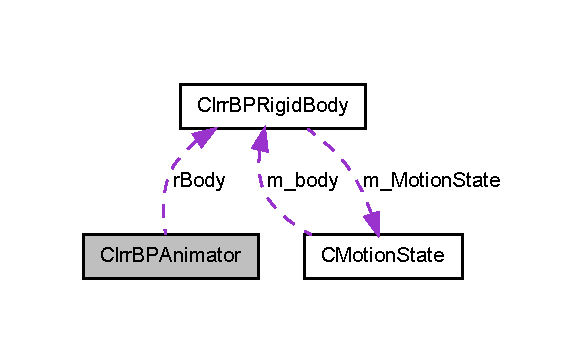
\includegraphics[width=190pt]{class_c_irr_b_p_animator__coll__graph}
\end{center}
\end{figure}
\subsection*{Public Member Functions}
\begin{DoxyCompactItemize}
\item 
\hypertarget{class_c_irr_b_p_animator_ac0c9f71966eb1f8a63138963a5a206d8}{
virtual void {\bfseries animate} ()=0}
\label{class_c_irr_b_p_animator_ac0c9f71966eb1f8a63138963a5a206d8}

\item 
\hypertarget{class_c_irr_b_p_animator_a9de50a01d583d29d8cd43a78f5b03050}{
virtual void {\bfseries drop} ()=0}
\label{class_c_irr_b_p_animator_a9de50a01d583d29d8cd43a78f5b03050}

\item 
\hypertarget{class_c_irr_b_p_animator_a2377f4311835330ee840d71f6f0989ea}{
virtual bool {\bfseries isEnd} ()}
\label{class_c_irr_b_p_animator_a2377f4311835330ee840d71f6f0989ea}

\item 
\hypertarget{class_c_irr_b_p_animator_add9c9e51946dfc2fb60876ed16c67441}{
virtual void {\bfseries setBody} (\hyperlink{class_c_irr_b_p_collision_object}{CIrrBPCollisionObject} $\ast$body)}
\label{class_c_irr_b_p_animator_add9c9e51946dfc2fb60876ed16c67441}

\end{DoxyCompactItemize}
\subsection*{Protected Attributes}
\begin{DoxyCompactItemize}
\item 
\hypertarget{class_c_irr_b_p_animator_a9b0924dd98d23c3d85f68b70e6f37032}{
\hyperlink{class_c_irr_b_p_collision_object}{CIrrBPCollisionObject} $\ast$ {\bfseries rBody}}
\label{class_c_irr_b_p_animator_a9b0924dd98d23c3d85f68b70e6f37032}

\item 
\hypertarget{class_c_irr_b_p_animator_a3b626ca4dc93b1496d66ce87f315c0ab}{
bool {\bfseries isEnded}}
\label{class_c_irr_b_p_animator_a3b626ca4dc93b1496d66ce87f315c0ab}

\end{DoxyCompactItemize}


The documentation for this class was generated from the following files:\begin{DoxyCompactItemize}
\item 
E:/Documenti/Lavori Stefano/ProgettoFPS/Engine/Engine/IrrBP/include/animator/CIrrBPAnimator.h\item 
E:/Documenti/Lavori Stefano/ProgettoFPS/Engine/Engine/IrrBP/src/animator/CIrrBPAnimator.cpp\end{DoxyCompactItemize}

\hypertarget{class_c_irr_b_p_box_body}{
\section{CIrrBPBoxBody Class Reference}
\label{class_c_irr_b_p_box_body}\index{CIrrBPBoxBody@{CIrrBPBoxBody}}
}


Inherits \hyperlink{class_c_irr_b_p_rigid_body}{CIrrBPRigidBody}.



Collaboration diagram for CIrrBPBoxBody:\nopagebreak
\begin{figure}[H]
\begin{center}
\leavevmode
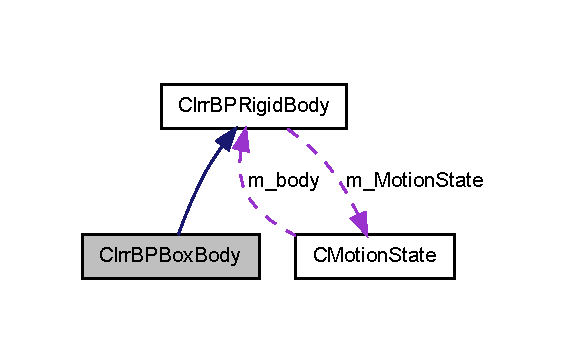
\includegraphics[width=273pt]{class_c_irr_b_p_box_body__coll__graph}
\end{center}
\end{figure}
\subsection*{Public Member Functions}
\begin{DoxyCompactItemize}
\item 
virtual void \hyperlink{class_c_irr_b_p_box_body_a144a57bdaaa418c5851f0beb97bdc44b}{drop} ()
\item 
\hypertarget{class_c_irr_b_p_box_body_a4deb7f0fd06fb982fa3815a3068f3a98}{
{\bfseries CIrrBPBoxBody} (ISceneNode $\ast$node, irr::f32 mass, irr::s32 bodyId=-\/1)}
\label{class_c_irr_b_p_box_body_a4deb7f0fd06fb982fa3815a3068f3a98}

\end{DoxyCompactItemize}


\subsection{Member Function Documentation}
\hypertarget{class_c_irr_b_p_box_body_a144a57bdaaa418c5851f0beb97bdc44b}{
\index{CIrrBPBoxBody@{CIrrBPBoxBody}!drop@{drop}}
\index{drop@{drop}!CIrrBPBoxBody@{CIrrBPBoxBody}}
\subsubsection[{drop}]{\setlength{\rightskip}{0pt plus 5cm}virtual void CIrrBPBoxBody::drop (
\begin{DoxyParamCaption}
{}
\end{DoxyParamCaption}
)\hspace{0.3cm}{\ttfamily  \mbox{[}inline, virtual\mbox{]}}}}
\label{class_c_irr_b_p_box_body_a144a57bdaaa418c5851f0beb97bdc44b}
Drop Function. This function should not be used. The destructor will be called automatically by the World Object. 

Implements \hyperlink{class_c_irr_b_p_rigid_body_a961d442e36e78260e7a6f203fd0c11e9}{CIrrBPRigidBody}.



The documentation for this class was generated from the following files:\begin{DoxyCompactItemize}
\item 
E:/Documenti/Lavori Stefano/ProgettoFPS/Engine/Engine/IrrBP/include/body/CIrrBPBoxBody.h\item 
E:/Documenti/Lavori Stefano/ProgettoFPS/Engine/Engine/IrrBP/src/body/CIrrBPBoxBody.cpp\end{DoxyCompactItemize}

\hypertarget{class_c_irr_b_p_capsule_body}{
\section{CIrrBPCapsuleBody Class Reference}
\label{class_c_irr_b_p_capsule_body}\index{CIrrBPCapsuleBody@{CIrrBPCapsuleBody}}
}


Inherits \hyperlink{class_c_irr_b_p_rigid_body}{CIrrBPRigidBody}.



Collaboration diagram for CIrrBPCapsuleBody:\nopagebreak
\begin{figure}[H]
\begin{center}
\leavevmode
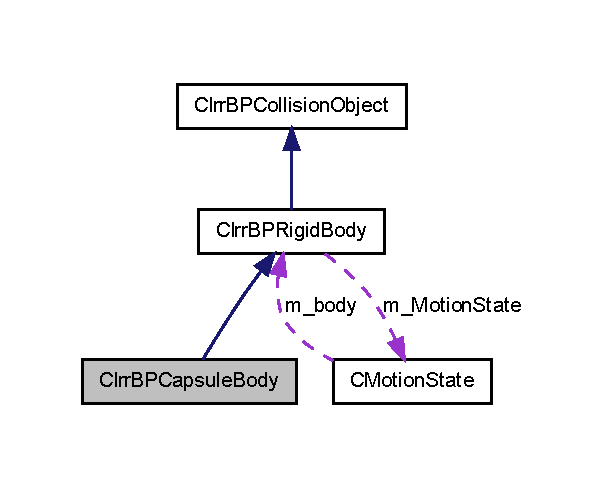
\includegraphics[width=291pt]{class_c_irr_b_p_capsule_body__coll__graph}
\end{center}
\end{figure}
\subsection*{Public Member Functions}
\begin{DoxyCompactItemize}
\item 
virtual void \hyperlink{class_c_irr_b_p_capsule_body_ab9815977583c6135b4b42dee8f536098}{drop} ()
\item 
\hypertarget{class_c_irr_b_p_capsule_body_a34a6ff788fddc82d0d9e7c836b6d38d3}{
{\bfseries CIrrBPCapsuleBody} (ISceneNode $\ast$node, irr::f32 mass, irr::s32 bodyId=-\/1, BODY\_\-OR bodyOrientationAxis=AUTO)}
\label{class_c_irr_b_p_capsule_body_a34a6ff788fddc82d0d9e7c836b6d38d3}

\end{DoxyCompactItemize}


\subsection{Member Function Documentation}
\hypertarget{class_c_irr_b_p_capsule_body_ab9815977583c6135b4b42dee8f536098}{
\index{CIrrBPCapsuleBody@{CIrrBPCapsuleBody}!drop@{drop}}
\index{drop@{drop}!CIrrBPCapsuleBody@{CIrrBPCapsuleBody}}
\subsubsection[{drop}]{\setlength{\rightskip}{0pt plus 5cm}virtual void CIrrBPCapsuleBody::drop (
\begin{DoxyParamCaption}
{}
\end{DoxyParamCaption}
)\hspace{0.3cm}{\ttfamily  \mbox{[}inline, virtual\mbox{]}}}}
\label{class_c_irr_b_p_capsule_body_ab9815977583c6135b4b42dee8f536098}
Drop Function. This function should not be used. The destructor will be called automatically by the World Object. 

Implements \hyperlink{class_c_irr_b_p_rigid_body_a961d442e36e78260e7a6f203fd0c11e9}{CIrrBPRigidBody}.



The documentation for this class was generated from the following files:\begin{DoxyCompactItemize}
\item 
E:/Documenti/Lavori Stefano/ProgettoFPS/Engine/Engine/IrrBP/include/body/CIrrBPCapsuleBody.h\item 
E:/Documenti/Lavori Stefano/ProgettoFPS/Engine/Engine/IrrBP/src/body/CIrrBPCapsuleBody.cpp\end{DoxyCompactItemize}

\hypertarget{class_c_irr_b_p_collision_delete_animator}{
\section{CIrrBPCollisionDeleteAnimator Class Reference}
\label{class_c_irr_b_p_collision_delete_animator}\index{CIrrBPCollisionDeleteAnimator@{CIrrBPCollisionDeleteAnimator}}
}


Please note that collision callback against soft body is not yet implemented in Bullet Physics.\par
 So The Collision Delete Animator DOESN'T works with soft bodies.  




{\ttfamily \#include $<$CIrrBPCollisionDeleteAnimator.h$>$}



Inherits \hyperlink{class_c_irr_b_p_animator}{CIrrBPAnimator}.



Collaboration diagram for CIrrBPCollisionDeleteAnimator:\nopagebreak
\begin{figure}[H]
\begin{center}
\leavevmode
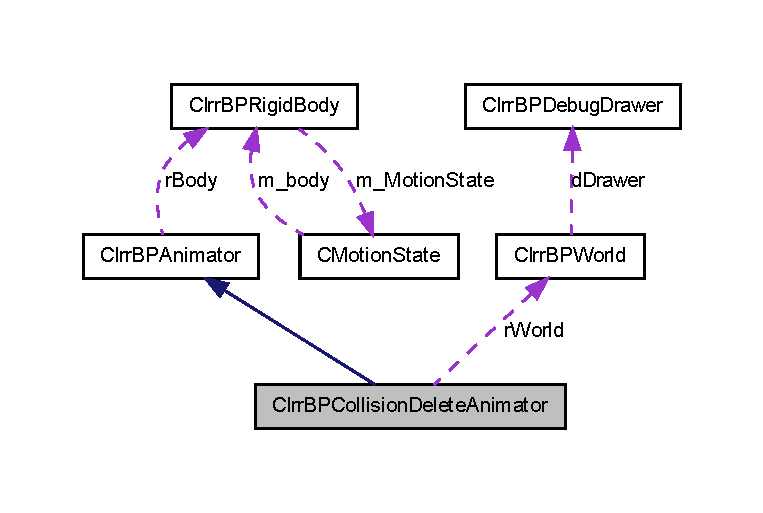
\includegraphics[width=310pt]{class_c_irr_b_p_collision_delete_animator__coll__graph}
\end{center}
\end{figure}
\subsection*{Public Member Functions}
\begin{DoxyCompactItemize}
\item 
\hypertarget{class_c_irr_b_p_collision_delete_animator_a4f097a814c55b2680acaa341e55aacc5}{
{\bfseries CIrrBPCollisionDeleteAnimator} (CIB\_\-DFLAG deleteFlag, \hyperlink{class_c_irr_b_p_world}{CIrrBPWorld} $\ast$world)}
\label{class_c_irr_b_p_collision_delete_animator_a4f097a814c55b2680acaa341e55aacc5}

\item 
\hypertarget{class_c_irr_b_p_collision_delete_animator_af69d93e6d128c6526ab8213ea69a63ab}{
void {\bfseries setBody} (\hyperlink{class_c_irr_b_p_collision_object}{CIrrBPCollisionObject} $\ast$body)}
\label{class_c_irr_b_p_collision_delete_animator_af69d93e6d128c6526ab8213ea69a63ab}

\item 
\hypertarget{class_c_irr_b_p_collision_delete_animator_a45e5e67fe3f214bcd0b12a29c657a2bf}{
void {\bfseries animate} ()}
\label{class_c_irr_b_p_collision_delete_animator_a45e5e67fe3f214bcd0b12a29c657a2bf}

\item 
\hypertarget{class_c_irr_b_p_collision_delete_animator_acbdbc88edb38bf253dcae6588574d95c}{
void {\bfseries drop} ()}
\label{class_c_irr_b_p_collision_delete_animator_acbdbc88edb38bf253dcae6588574d95c}

\end{DoxyCompactItemize}


\subsection{Detailed Description}
Please note that collision callback against soft body is not yet implemented in Bullet Physics.\par
 So The Collision Delete Animator DOESN'T works with soft bodies. 

The documentation for this class was generated from the following files:\begin{DoxyCompactItemize}
\item 
E:/Documenti/Lavori Stefano/ProgettoFPS/Engine/Engine/IrrBP/include/animator/CIrrBPCollisionDeleteAnimator.h\item 
E:/Documenti/Lavori Stefano/ProgettoFPS/Engine/Engine/IrrBP/src/animator/CIrrBPCollisionDeleteAnimator.cpp\end{DoxyCompactItemize}

\hypertarget{class_c_irr_b_p_cone_body}{
\section{CIrrBPConeBody Class Reference}
\label{class_c_irr_b_p_cone_body}\index{CIrrBPConeBody@{CIrrBPConeBody}}
}


Inherits \hyperlink{class_c_irr_b_p_rigid_body}{CIrrBPRigidBody}.



Collaboration diagram for CIrrBPConeBody:\nopagebreak
\begin{figure}[H]
\begin{center}
\leavevmode
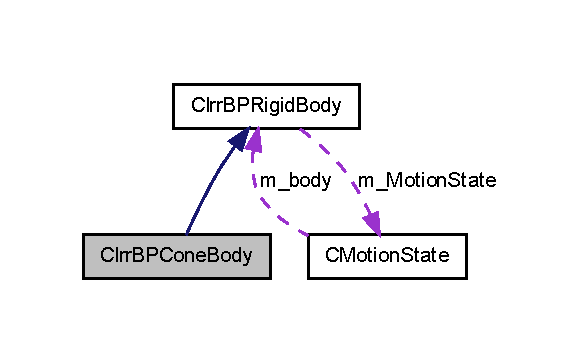
\includegraphics[width=279pt]{class_c_irr_b_p_cone_body__coll__graph}
\end{center}
\end{figure}
\subsection*{Public Member Functions}
\begin{DoxyCompactItemize}
\item 
virtual void \hyperlink{class_c_irr_b_p_cone_body_a47470fa549f852a5d315f0decb4d195a}{drop} ()
\item 
\hypertarget{class_c_irr_b_p_cone_body_acda43501a8f1826103caf9a925ba229c}{
{\bfseries CIrrBPConeBody} (ISceneNode $\ast$node, irr::f32 mass, irr::s32 bodyId=-\/1, BODY\_\-OR bodyOrientationAxis=AUTO)}
\label{class_c_irr_b_p_cone_body_acda43501a8f1826103caf9a925ba229c}

\end{DoxyCompactItemize}


\subsection{Member Function Documentation}
\hypertarget{class_c_irr_b_p_cone_body_a47470fa549f852a5d315f0decb4d195a}{
\index{CIrrBPConeBody@{CIrrBPConeBody}!drop@{drop}}
\index{drop@{drop}!CIrrBPConeBody@{CIrrBPConeBody}}
\subsubsection[{drop}]{\setlength{\rightskip}{0pt plus 5cm}virtual void CIrrBPConeBody::drop (
\begin{DoxyParamCaption}
{}
\end{DoxyParamCaption}
)\hspace{0.3cm}{\ttfamily  \mbox{[}inline, virtual\mbox{]}}}}
\label{class_c_irr_b_p_cone_body_a47470fa549f852a5d315f0decb4d195a}
Drop Function. This function should not be used. The destructor will be called automatically by the World Object. 

Implements \hyperlink{class_c_irr_b_p_rigid_body_a961d442e36e78260e7a6f203fd0c11e9}{CIrrBPRigidBody}.



The documentation for this class was generated from the following files:\begin{DoxyCompactItemize}
\item 
E:/Documenti/Lavori Stefano/ProgettoFPS/Engine/Engine/IrrBP/include/body/CIrrBPConeBody.h\item 
E:/Documenti/Lavori Stefano/ProgettoFPS/Engine/Engine/IrrBP/src/body/CIrrBPConeBody.cpp\end{DoxyCompactItemize}

\hypertarget{class_c_irr_b_p_cone_twist_constraint}{
\section{CIrrBPConeTwistConstraint Class Reference}
\label{class_c_irr_b_p_cone_twist_constraint}\index{CIrrBPConeTwistConstraint@{CIrrBPConeTwistConstraint}}
}


Inherits \hyperlink{class_c_irr_b_p_constraint}{CIrrBPConstraint}.



Collaboration diagram for CIrrBPConeTwistConstraint:\nopagebreak
\begin{figure}[H]
\begin{center}
\leavevmode
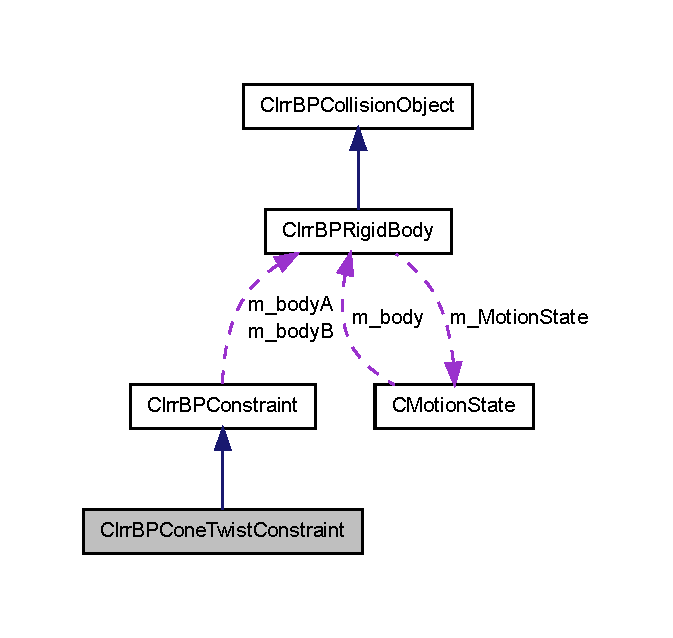
\includegraphics[width=323pt]{class_c_irr_b_p_cone_twist_constraint__coll__graph}
\end{center}
\end{figure}
\subsection*{Public Member Functions}
\begin{DoxyCompactItemize}
\item 
\hypertarget{class_c_irr_b_p_cone_twist_constraint_a7d1dc01fc82710be739ac816e370b627}{
{\bfseries CIrrBPConeTwistConstraint} (\hyperlink{class_c_irr_b_p_rigid_body}{CIrrBPRigidBody} $\ast$bodyA, \hyperlink{class_c_irr_b_p_rigid_body}{CIrrBPRigidBody} $\ast$bodyB, const vector3df \&pivotInA=vector3df(0, 0, 0), const vector3df \&pivotInB=vector3df(0, 0, 0))}
\label{class_c_irr_b_p_cone_twist_constraint_a7d1dc01fc82710be739ac816e370b627}

\item 
void \hyperlink{class_c_irr_b_p_cone_twist_constraint_a11ae1560c750788403c260ba82f9b02e}{drop} ()
\item 
\hypertarget{class_c_irr_b_p_cone_twist_constraint_a3d93592e31b2bd9cbb64d6dfb54e6fe9}{
void {\bfseries setLimit} (int limitIndex, irr::f32 limitValue)}
\label{class_c_irr_b_p_cone_twist_constraint_a3d93592e31b2bd9cbb64d6dfb54e6fe9}

\item 
\hypertarget{class_c_irr_b_p_cone_twist_constraint_af01718483b71e61db51393427e7a752f}{
void {\bfseries setLimit} (irr::f32 \_\-swingSpan1, irr::f32 \_\-swingSpan2, irr::f32 \_\-twistSpan, irr::f32 \_\-softness=1.f, irr::f32 \_\-biasFactor=0.3f, irr::f32 \_\-relaxationFactor=1.0f)}
\label{class_c_irr_b_p_cone_twist_constraint_af01718483b71e61db51393427e7a752f}

\end{DoxyCompactItemize}


\subsection{Member Function Documentation}
\hypertarget{class_c_irr_b_p_cone_twist_constraint_a11ae1560c750788403c260ba82f9b02e}{
\index{CIrrBPConeTwistConstraint@{CIrrBPConeTwistConstraint}!drop@{drop}}
\index{drop@{drop}!CIrrBPConeTwistConstraint@{CIrrBPConeTwistConstraint}}
\subsubsection[{drop}]{\setlength{\rightskip}{0pt plus 5cm}void CIrrBPConeTwistConstraint::drop (
\begin{DoxyParamCaption}
{}
\end{DoxyParamCaption}
)\hspace{0.3cm}{\ttfamily  \mbox{[}inline, virtual\mbox{]}}}}
\label{class_c_irr_b_p_cone_twist_constraint_a11ae1560c750788403c260ba82f9b02e}
Drop Function. This function should not be used. The destructor will be called automatically by the World Object. 

Implements \hyperlink{class_c_irr_b_p_constraint_a2718ef7118d60646a5cfa2dfe5a44795}{CIrrBPConstraint}.



The documentation for this class was generated from the following files:\begin{DoxyCompactItemize}
\item 
E:/Documenti/Lavori Stefano/ProgettoFPS/Engine/Engine/IrrBP/include/constraint/CIrrBPConeTwistConstraint.h\item 
E:/Documenti/Lavori Stefano/ProgettoFPS/Engine/Engine/IrrBP/src/constraint/CIrrBPConeTwistConstraint.cpp\end{DoxyCompactItemize}

\hypertarget{class_c_irr_b_p_constraint}{
\section{CIrrBPConstraint Class Reference}
\label{class_c_irr_b_p_constraint}\index{CIrrBPConstraint@{CIrrBPConstraint}}
}


Inherited by \hyperlink{class_c_irr_b_p_hinge_constraint}{CIrrBPHingeConstraint}, \hyperlink{class_c_irr_b_p_p2_p_constraint}{CIrrBPP2PConstraint}, and \hyperlink{class_c_irr_b_p_slide_constraint}{CIrrBPSlideConstraint}.



Collaboration diagram for CIrrBPConstraint:\nopagebreak
\begin{figure}[H]
\begin{center}
\leavevmode
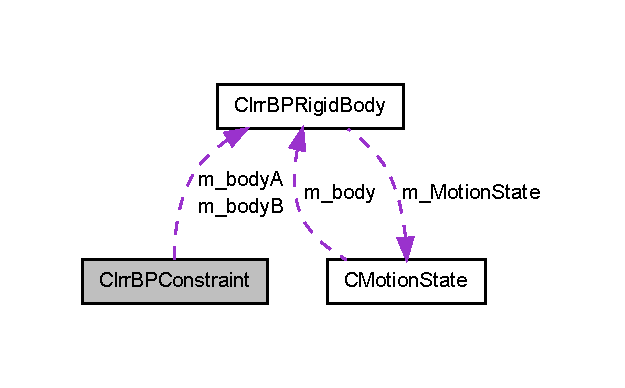
\includegraphics[width=300pt]{class_c_irr_b_p_constraint__coll__graph}
\end{center}
\end{figure}
\subsection*{Public Member Functions}
\begin{DoxyCompactItemize}
\item 
virtual void \hyperlink{class_c_irr_b_p_constraint_a2718ef7118d60646a5cfa2dfe5a44795}{drop} ()=0
\item 
\hypertarget{class_c_irr_b_p_constraint_acfb5d4e8b25c91e150af372f4bd9187e}{
btTypedConstraint $\ast$ {\bfseries getConstraintPtr} ()}
\label{class_c_irr_b_p_constraint_acfb5d4e8b25c91e150af372f4bd9187e}

\item 
\hypertarget{class_c_irr_b_p_constraint_ac109e0c136271d9c002c5521a2eacc15}{
\hyperlink{class_c_irr_b_p_rigid_body}{CIrrBPRigidBody} $\ast$ {\bfseries getBodyA} ()}
\label{class_c_irr_b_p_constraint_ac109e0c136271d9c002c5521a2eacc15}

\item 
\hypertarget{class_c_irr_b_p_constraint_a0774899cfd927b7dcf7d1ab45552c122}{
\hyperlink{class_c_irr_b_p_rigid_body}{CIrrBPRigidBody} $\ast$ {\bfseries getBodyB} ()}
\label{class_c_irr_b_p_constraint_a0774899cfd927b7dcf7d1ab45552c122}

\end{DoxyCompactItemize}
\subsection*{Protected Attributes}
\begin{DoxyCompactItemize}
\item 
\hypertarget{class_c_irr_b_p_constraint_ad755c2f634eea7261b5bf8b352299977}{
btTypedConstraint $\ast$ {\bfseries m\_\-Constraint}}
\label{class_c_irr_b_p_constraint_ad755c2f634eea7261b5bf8b352299977}

\item 
\hypertarget{class_c_irr_b_p_constraint_ae300a6d42c498864fce18eb2cc4f85ec}{
\hyperlink{class_c_irr_b_p_rigid_body}{CIrrBPRigidBody} $\ast$ {\bfseries m\_\-bodyA}}
\label{class_c_irr_b_p_constraint_ae300a6d42c498864fce18eb2cc4f85ec}

\item 
\hypertarget{class_c_irr_b_p_constraint_ab5ee9998be891258f78badd48702f101}{
vector3df {\bfseries m\_\-pivotA}}
\label{class_c_irr_b_p_constraint_ab5ee9998be891258f78badd48702f101}

\item 
\hypertarget{class_c_irr_b_p_constraint_ae9848f0a6e9b036c0720b6114a501cc1}{
\hyperlink{class_c_irr_b_p_rigid_body}{CIrrBPRigidBody} $\ast$ {\bfseries m\_\-bodyB}}
\label{class_c_irr_b_p_constraint_ae9848f0a6e9b036c0720b6114a501cc1}

\item 
\hypertarget{class_c_irr_b_p_constraint_a573ccefffed59ecff42a2ab1b71b3724}{
vector3df {\bfseries m\_\-pivotB}}
\label{class_c_irr_b_p_constraint_a573ccefffed59ecff42a2ab1b71b3724}

\end{DoxyCompactItemize}


\subsection{Member Function Documentation}
\hypertarget{class_c_irr_b_p_constraint_a2718ef7118d60646a5cfa2dfe5a44795}{
\index{CIrrBPConstraint@{CIrrBPConstraint}!drop@{drop}}
\index{drop@{drop}!CIrrBPConstraint@{CIrrBPConstraint}}
\subsubsection[{drop}]{\setlength{\rightskip}{0pt plus 5cm}virtual void CIrrBPConstraint::drop (
\begin{DoxyParamCaption}
{}
\end{DoxyParamCaption}
)\hspace{0.3cm}{\ttfamily  \mbox{[}pure virtual\mbox{]}}}}
\label{class_c_irr_b_p_constraint_a2718ef7118d60646a5cfa2dfe5a44795}
Drop Function. This function should not be used. The destructor will be called automatically by the World Object. 

Implemented in \hyperlink{class_c_irr_b_p_hinge_constraint_a8c9ba8b2ee3bdff9ea684f2200c302ce}{CIrrBPHingeConstraint}, \hyperlink{class_c_irr_b_p_p2_p_constraint_abc3ec07fbc260cb8f88727fd8e9fc2c6}{CIrrBPP2PConstraint}, and \hyperlink{class_c_irr_b_p_slide_constraint_acaaf3cfaba14b8c126ab548f7c21c2b6}{CIrrBPSlideConstraint}.



The documentation for this class was generated from the following files:\begin{DoxyCompactItemize}
\item 
E:/Documenti/Lavori Stefano/ProgettoFPS/Engine/Engine/IrrBP/include/constraint/CIrrBPConstraint.h\item 
E:/Documenti/Lavori Stefano/ProgettoFPS/Engine/Engine/IrrBP/src/constraint/CIrrBPConstraint.cpp\end{DoxyCompactItemize}

\hypertarget{class_c_irr_b_p_cylinder_body}{
\section{CIrrBPCylinderBody Class Reference}
\label{class_c_irr_b_p_cylinder_body}\index{CIrrBPCylinderBody@{CIrrBPCylinderBody}}
}


Inherits \hyperlink{class_c_irr_b_p_rigid_body}{CIrrBPRigidBody}.



Collaboration diagram for CIrrBPCylinderBody:\nopagebreak
\begin{figure}[H]
\begin{center}
\leavevmode
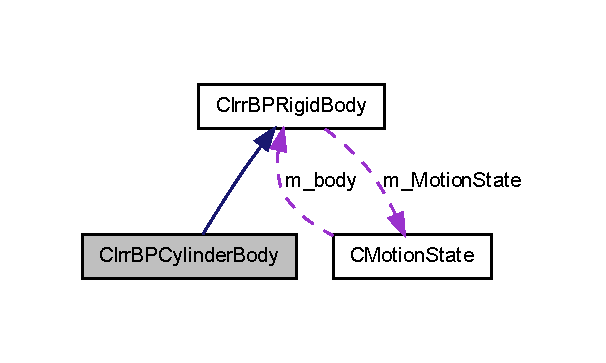
\includegraphics[width=291pt]{class_c_irr_b_p_cylinder_body__coll__graph}
\end{center}
\end{figure}
\subsection*{Public Member Functions}
\begin{DoxyCompactItemize}
\item 
virtual void \hyperlink{class_c_irr_b_p_cylinder_body_a966bec7330f778f276294601fc7e0c45}{drop} ()
\item 
\hypertarget{class_c_irr_b_p_cylinder_body_a6eb977e0589946de5beb42f4a1c74900}{
{\bfseries CIrrBPCylinderBody} (ISceneNode $\ast$node, irr::f32 mass, irr::s32 bodyId=-\/1, BODY\_\-OR bodyOrientationAxis=AUTO)}
\label{class_c_irr_b_p_cylinder_body_a6eb977e0589946de5beb42f4a1c74900}

\end{DoxyCompactItemize}


\subsection{Member Function Documentation}
\hypertarget{class_c_irr_b_p_cylinder_body_a966bec7330f778f276294601fc7e0c45}{
\index{CIrrBPCylinderBody@{CIrrBPCylinderBody}!drop@{drop}}
\index{drop@{drop}!CIrrBPCylinderBody@{CIrrBPCylinderBody}}
\subsubsection[{drop}]{\setlength{\rightskip}{0pt plus 5cm}virtual void CIrrBPCylinderBody::drop (
\begin{DoxyParamCaption}
{}
\end{DoxyParamCaption}
)\hspace{0.3cm}{\ttfamily  \mbox{[}inline, virtual\mbox{]}}}}
\label{class_c_irr_b_p_cylinder_body_a966bec7330f778f276294601fc7e0c45}
Drop Function. This function should not be used. The destructor will be called automatically by the World Object. 

Implements \hyperlink{class_c_irr_b_p_rigid_body_a961d442e36e78260e7a6f203fd0c11e9}{CIrrBPRigidBody}.



The documentation for this class was generated from the following files:\begin{DoxyCompactItemize}
\item 
E:/Documenti/Lavori Stefano/ProgettoFPS/Engine/Engine/IrrBP/include/body/CIrrBPCylinderBody.h\item 
E:/Documenti/Lavori Stefano/ProgettoFPS/Engine/Engine/IrrBP/src/body/CIrrBPCylinderBody.cpp\end{DoxyCompactItemize}

\hypertarget{class_c_irr_b_p_debug_drawer}{
\section{CIrrBPDebugDrawer Class Reference}
\label{class_c_irr_b_p_debug_drawer}\index{CIrrBPDebugDrawer@{CIrrBPDebugDrawer}}
}


Should not be used. Only for internal use.  




{\ttfamily \#include $<$CIrrBPDebugDrawer.h$>$}

\subsection*{Public Member Functions}
\begin{DoxyCompactItemize}
\item 
\hypertarget{class_c_irr_b_p_debug_drawer_a5b14a017628afd8f1a6e6bcdc6ad6e5d}{
{\bfseries CIrrBPDebugDrawer} (irr::video::IVideoDriver $\ast$driver)}
\label{class_c_irr_b_p_debug_drawer_a5b14a017628afd8f1a6e6bcdc6ad6e5d}

\item 
\hypertarget{class_c_irr_b_p_debug_drawer_a658c524baf35bc7546228e9de858624a}{
void {\bfseries drawLine} (const btVector3 \&from, const btVector3 \&to, const btVector3 \&color)}
\label{class_c_irr_b_p_debug_drawer_a658c524baf35bc7546228e9de858624a}

\item 
\hypertarget{class_c_irr_b_p_debug_drawer_acefdd7e7736d328b811b0b13b1031d20}{
void {\bfseries drawTriangle} (const btVector3 \&v0, const btVector3 \&v1, const btVector3 \&v2, const btVector3 \&color, btScalar alpha)}
\label{class_c_irr_b_p_debug_drawer_acefdd7e7736d328b811b0b13b1031d20}

\item 
\hypertarget{class_c_irr_b_p_debug_drawer_a2b2c18c0eb12653a9a6f01ad65fb73b7}{
void {\bfseries drawContactPoint} (const btVector3 \&PointOnB, const btVector3 \&normalOnB, btScalar distance, int lifeTime, const btVector3 \&color)}
\label{class_c_irr_b_p_debug_drawer_a2b2c18c0eb12653a9a6f01ad65fb73b7}

\item 
\hypertarget{class_c_irr_b_p_debug_drawer_a9084e5b734e0e7ad507c80fe164af765}{
void {\bfseries reportErrorWarning} (const char $\ast$text)}
\label{class_c_irr_b_p_debug_drawer_a9084e5b734e0e7ad507c80fe164af765}

\item 
\hypertarget{class_c_irr_b_p_debug_drawer_a6279d86e4d91611ade0313f5644041ad}{
void {\bfseries draw3dText} (const btVector3 \&location, const char $\ast$text)}
\label{class_c_irr_b_p_debug_drawer_a6279d86e4d91611ade0313f5644041ad}

\item 
\hypertarget{class_c_irr_b_p_debug_drawer_ac0c787365db5b827e4c461ec11a4be07}{
void {\bfseries setDebugMode} (int mode)}
\label{class_c_irr_b_p_debug_drawer_ac0c787365db5b827e4c461ec11a4be07}

\item 
\hypertarget{class_c_irr_b_p_debug_drawer_af195b57e20e31c217fd9b410c8b73a4f}{
int {\bfseries getDebugMode} () const }
\label{class_c_irr_b_p_debug_drawer_af195b57e20e31c217fd9b410c8b73a4f}

\end{DoxyCompactItemize}


\subsection{Detailed Description}
Should not be used. Only for internal use. 

The documentation for this class was generated from the following files:\begin{DoxyCompactItemize}
\item 
E:/Documenti/Lavori Stefano/ProgettoFPS/Engine/Engine/IrrBP/include/CIrrBPDebugDrawer.h\item 
E:/Documenti/Lavori Stefano/ProgettoFPS/Engine/Engine/IrrBP/src/CIrrBPDebugDrawer.cpp\end{DoxyCompactItemize}

\hypertarget{class_c_irr_b_p_delete_animator}{
\section{CIrrBPDeleteAnimator Class Reference}
\label{class_c_irr_b_p_delete_animator}\index{CIrrBPDeleteAnimator@{CIrrBPDeleteAnimator}}
}


Inherits \hyperlink{class_c_irr_b_p_animator}{CIrrBPAnimator}.



Collaboration diagram for CIrrBPDeleteAnimator:\nopagebreak
\begin{figure}[H]
\begin{center}
\leavevmode
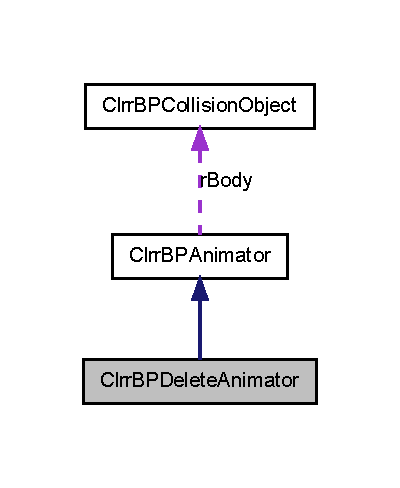
\includegraphics[width=295pt]{class_c_irr_b_p_delete_animator__coll__graph}
\end{center}
\end{figure}
\subsection*{Public Member Functions}
\begin{DoxyCompactItemize}
\item 
\hypertarget{class_c_irr_b_p_delete_animator_a2eef152cff22579d3c706a2444b611ec}{
{\bfseries CIrrBPDeleteAnimator} (ITimer $\ast$timer, irr::u32 end)}
\label{class_c_irr_b_p_delete_animator_a2eef152cff22579d3c706a2444b611ec}

\item 
\hypertarget{class_c_irr_b_p_delete_animator_a0ff69f375c5a499c7d07e81bc93168a3}{
void {\bfseries setBody} (\hyperlink{class_c_irr_b_p_rigid_body}{CIrrBPRigidBody} $\ast$body)}
\label{class_c_irr_b_p_delete_animator_a0ff69f375c5a499c7d07e81bc93168a3}

\item 
\hypertarget{class_c_irr_b_p_delete_animator_a41ce1c90f4f4f316e3a08a5a431a5769}{
void {\bfseries animate} ()}
\label{class_c_irr_b_p_delete_animator_a41ce1c90f4f4f316e3a08a5a431a5769}

\item 
\hypertarget{class_c_irr_b_p_delete_animator_a10fcff4d2fd949ea59596a827a76a057}{
void {\bfseries drop} ()}
\label{class_c_irr_b_p_delete_animator_a10fcff4d2fd949ea59596a827a76a057}

\end{DoxyCompactItemize}


The documentation for this class was generated from the following files:\begin{DoxyCompactItemize}
\item 
E:/Documenti/Lavori Stefano/ProgettoFPS/Engine/Engine/IrrBP/include/animator/CIrrBPDeleteAnimator.h\item 
E:/Documenti/Lavori Stefano/ProgettoFPS/Engine/Engine/IrrBP/src/animator/CIrrBPDeleteAnimator.cpp\end{DoxyCompactItemize}

\hypertarget{class_c_irr_b_p_hinge_constraint}{
\section{CIrrBPHingeConstraint Class Reference}
\label{class_c_irr_b_p_hinge_constraint}\index{CIrrBPHingeConstraint@{CIrrBPHingeConstraint}}
}


Inherits \hyperlink{class_c_irr_b_p_constraint}{CIrrBPConstraint}.



Collaboration diagram for CIrrBPHingeConstraint:\nopagebreak
\begin{figure}[H]
\begin{center}
\leavevmode
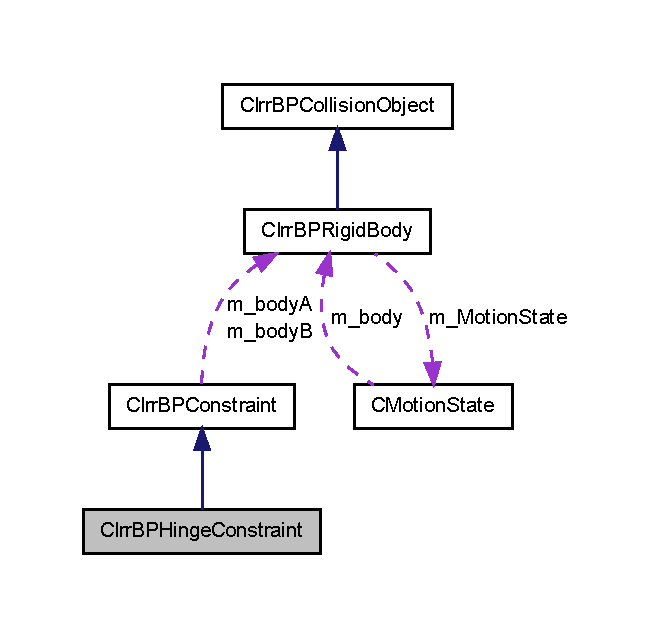
\includegraphics[width=313pt]{class_c_irr_b_p_hinge_constraint__coll__graph}
\end{center}
\end{figure}
\subsection*{Public Member Functions}
\begin{DoxyCompactItemize}
\item 
\hypertarget{class_c_irr_b_p_hinge_constraint_affb8842f43c680b6d1e86a393e7bca85}{
{\bfseries CIrrBPHingeConstraint} (\hyperlink{class_c_irr_b_p_rigid_body}{CIrrBPRigidBody} $\ast$bodyA, const vector3df \&pivotInA, const vector3df \&axisInA)}
\label{class_c_irr_b_p_hinge_constraint_affb8842f43c680b6d1e86a393e7bca85}

\item 
\hypertarget{class_c_irr_b_p_hinge_constraint_a454755a449d4d86e0904ee51aade72ec}{
{\bfseries CIrrBPHingeConstraint} (\hyperlink{class_c_irr_b_p_rigid_body}{CIrrBPRigidBody} $\ast$bodyA, \hyperlink{class_c_irr_b_p_rigid_body}{CIrrBPRigidBody} $\ast$bodyB, const vector3df \&pivotInA, const vector3df \&pivotInB, const vector3df \&axisInA, const vector3df \&axisInB)}
\label{class_c_irr_b_p_hinge_constraint_a454755a449d4d86e0904ee51aade72ec}

\item 
void \hyperlink{class_c_irr_b_p_hinge_constraint_a8c9ba8b2ee3bdff9ea684f2200c302ce}{drop} ()
\end{DoxyCompactItemize}
\subsection*{Protected Attributes}
\begin{DoxyCompactItemize}
\item 
\hypertarget{class_c_irr_b_p_hinge_constraint_abcdcdf37670d468b67b14efa37c22c00}{
vector3df {\bfseries m\_\-axisA}}
\label{class_c_irr_b_p_hinge_constraint_abcdcdf37670d468b67b14efa37c22c00}

\item 
\hypertarget{class_c_irr_b_p_hinge_constraint_a3ad3f250f5b9df9d91231d9f8e4abb0e}{
vector3df {\bfseries m\_\-axisB}}
\label{class_c_irr_b_p_hinge_constraint_a3ad3f250f5b9df9d91231d9f8e4abb0e}

\end{DoxyCompactItemize}


\subsection{Member Function Documentation}
\hypertarget{class_c_irr_b_p_hinge_constraint_a8c9ba8b2ee3bdff9ea684f2200c302ce}{
\index{CIrrBPHingeConstraint@{CIrrBPHingeConstraint}!drop@{drop}}
\index{drop@{drop}!CIrrBPHingeConstraint@{CIrrBPHingeConstraint}}
\subsubsection[{drop}]{\setlength{\rightskip}{0pt plus 5cm}void CIrrBPHingeConstraint::drop (
\begin{DoxyParamCaption}
{}
\end{DoxyParamCaption}
)\hspace{0.3cm}{\ttfamily  \mbox{[}inline, virtual\mbox{]}}}}
\label{class_c_irr_b_p_hinge_constraint_a8c9ba8b2ee3bdff9ea684f2200c302ce}
Drop Function. This function should not be used. The destructor will be called automatically by the World Object. 

Implements \hyperlink{class_c_irr_b_p_constraint_a2718ef7118d60646a5cfa2dfe5a44795}{CIrrBPConstraint}.



The documentation for this class was generated from the following files:\begin{DoxyCompactItemize}
\item 
E:/Documenti/Lavori Stefano/ProgettoFPS/Engine/Engine/IrrBP/include/constraint/CIrrBPHingeConstraint.h\item 
E:/Documenti/Lavori Stefano/ProgettoFPS/Engine/Engine/IrrBP/src/constraint/CIrrBPHingeConstraint.cpp\end{DoxyCompactItemize}

\hypertarget{class_c_irr_b_p_manager}{
\section{CIrrBPManager Class Reference}
\label{class_c_irr_b_p_manager}\index{CIrrBPManager@{CIrrBPManager}}
}


Collaboration diagram for CIrrBPManager:\nopagebreak
\begin{figure}[H]
\begin{center}
\leavevmode
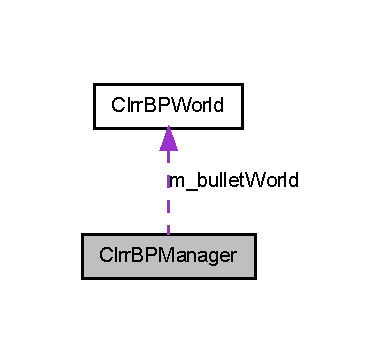
\includegraphics[width=194pt]{class_c_irr_b_p_manager__coll__graph}
\end{center}
\end{figure}
\subsection*{Public Member Functions}
\begin{DoxyCompactItemize}
\item 
\hyperlink{class_c_irr_b_p_manager_ae449dd7e0fa17f986a8ee2b6afe36a09}{CIrrBPManager} (IrrlichtDevice $\ast$device)
\item 
\hyperlink{class_c_irr_b_p_world}{CIrrBPWorld} $\ast$ \hyperlink{class_c_irr_b_p_manager_acdfaf5f8c351d72c4d9680cb75372ae3}{getWorld} ()
\item 
\hyperlink{class_c_irr_b_p_box_body}{CIrrBPBoxBody} $\ast$ \hyperlink{class_c_irr_b_p_manager_a61ed9d76cfe90285f6e7d80b5870406f}{addRigidBox} (ISceneNode $\ast$node, irr::f32 mass, irr::s32 bodyId=-\/1)
\item 
\hyperlink{class_c_irr_b_p_sphere_body}{CIrrBPSphereBody} $\ast$ \hyperlink{class_c_irr_b_p_manager_aebbe19de8a748a7c66d5d0efc16dc5eb}{addRigidSphere} (ISceneNode $\ast$node, irr::f32 mass, irr::s32 bodyId=-\/1)
\item 
\hyperlink{class_c_irr_b_p_cylinder_body}{CIrrBPCylinderBody} $\ast$ \hyperlink{class_c_irr_b_p_manager_a7866f42ff533e69342c9ad370f07aa23}{addRigidCylinder} (ISceneNode $\ast$node, irr::f32 mass, irr::s32 bodyId=-\/1, BODY\_\-OR bodyOrientationAxis=AUTO)
\item 
\hyperlink{class_c_irr_b_p_cone_body}{CIrrBPConeBody} $\ast$ \hyperlink{class_c_irr_b_p_manager_a810377e264480789138dc4b9ac5145d4}{addRigidCone} (ISceneNode $\ast$node, irr::f32 mass, irr::s32 bodyId=-\/1, BODY\_\-OR bodyOrientationAxis=AUTO)
\item 
\hyperlink{class_c_irr_b_p_capsule_body}{CIrrBPCapsuleBody} $\ast$ \hyperlink{class_c_irr_b_p_manager_ac351ba81cf28a33bac69bc348860cd48}{addRigidCapsule} (ISceneNode $\ast$node, irr::f32 mass, irr::s32 bodyId=-\/1, BODY\_\-OR bodyOrientationAxis=AUTO)
\item 
\hyperlink{class_c_irr_b_p_trimesh}{CIrrBPTrimesh} $\ast$ \hyperlink{class_c_irr_b_p_manager_ad565fee43722307839908de9aab70344}{addTrimesh} (IAnimatedMeshSceneNode $\ast$node, irr::f32 mass, irr::s32 bodyId=-\/1)
\item 
\hyperlink{class_c_irr_b_p_trimesh}{CIrrBPTrimesh} $\ast$ \hyperlink{class_c_irr_b_p_manager_a14eef4c19ac93cf7dff82544637833e0}{addTrimesh} (IMeshSceneNode $\ast$node, irr::f32 mass, irr::s32 bodyId=-\/1)
\item 
\hyperlink{class_c_irr_b_p_slide_constraint}{CIrrBPSlideConstraint} $\ast$ \hyperlink{class_c_irr_b_p_manager_af916152de29ba8c7c9e727dfe5a1c8af}{buildSlideConstraint} (\hyperlink{class_c_irr_b_p_rigid_body}{CIrrBPRigidBody} $\ast$bodyA, \hyperlink{class_c_irr_b_p_rigid_body}{CIrrBPRigidBody} $\ast$bodyB, const vector3df \&pivotInA=vector3df(0, 0, 0), const vector3df \&pivotInB=vector3df(0, 0, 0), bool autoadapt=true, bool rotatepiston=true)
\item 
\hyperlink{class_c_irr_b_p_p2_p_constraint}{CIrrBPP2PConstraint} $\ast$ \hyperlink{class_c_irr_b_p_manager_a19a7a9108ded5c076d307efdb390d58a}{buildP2PConstraint} (\hyperlink{class_c_irr_b_p_rigid_body}{CIrrBPRigidBody} $\ast$bodyA, const vector3df \&pivotInA=vector3df(0, 0, 0))
\item 
\hyperlink{class_c_irr_b_p_p2_p_constraint}{CIrrBPP2PConstraint} $\ast$ \hyperlink{class_c_irr_b_p_manager_a1a2dc64a93a8770dfed3ba7f77972c70}{buildP2PConstraint} (\hyperlink{class_c_irr_b_p_rigid_body}{CIrrBPRigidBody} $\ast$bodyA, \hyperlink{class_c_irr_b_p_rigid_body}{CIrrBPRigidBody} $\ast$bodyB, const vector3df \&pivotInA=vector3df(0, 0, 0), const vector3df \&pivotInB=vector3df(0, 0, 0))
\item 
\hyperlink{class_c_irr_b_p_cone_twist_constraint}{CIrrBPConeTwistConstraint} $\ast$ \hyperlink{class_c_irr_b_p_manager_ae6c1ebbc11dec61a856bcc7b5c6394ce}{buildConeTwistConstraint} (\hyperlink{class_c_irr_b_p_rigid_body}{CIrrBPRigidBody} $\ast$bodyA, \hyperlink{class_c_irr_b_p_rigid_body}{CIrrBPRigidBody} $\ast$bodyB, const vector3df \&pivotInA=vector3df(0, 0, 0), const vector3df \&pivotInB=vector3df(0, 0, 0))
\item 
\hyperlink{class_c_irr_b_p_hinge_constraint}{CIrrBPHingeConstraint} $\ast$ \hyperlink{class_c_irr_b_p_manager_a87b2610eaba14775ac81992ff71ab436}{buildHingeConstraint} (\hyperlink{class_c_irr_b_p_rigid_body}{CIrrBPRigidBody} $\ast$bodyA, const vector3df \&pivotInA, const vector3df \&axisInA)
\item 
\hyperlink{class_c_irr_b_p_hinge_constraint}{CIrrBPHingeConstraint} $\ast$ \hyperlink{class_c_irr_b_p_manager_a8a61e921b487d6249e46022b6e9b5ccf}{buildHingeConstraint} (\hyperlink{class_c_irr_b_p_rigid_body}{CIrrBPRigidBody} $\ast$bodyA, \hyperlink{class_c_irr_b_p_rigid_body}{CIrrBPRigidBody} $\ast$bodyB, const vector3df \&pivotInA, const vector3df \&pivotInB, const vector3df \&axisInA, const vector3df \&axisInB)
\item 
\hyperlink{class_c_irr_b_p_delete_animator}{CIrrBPDeleteAnimator} $\ast$ \hyperlink{class_c_irr_b_p_manager_a34d992b091c917aa9a0febddadf26141}{createDeleteAnimator} (irr::u32 timeMs)
\item 
\hyperlink{class_c_irr_b_p_collision_delete_animator}{CIrrBPCollisionDeleteAnimator} $\ast$ \hyperlink{class_c_irr_b_p_manager_a868af77531e0eb62d14ee060d2c91158}{createCollisionDeleteAnimator} (CIB\_\-DFLAG delFlag)
\item 
void \hyperlink{class_c_irr_b_p_manager_af5b96f07769449e5b4a7adb8485e027f}{addBodyToBulletQueue} (\hyperlink{class_c_irr_b_p_rigid_body}{CIrrBPRigidBody} $\ast$body)
\item 
void \hyperlink{class_c_irr_b_p_manager_ad4896d9448a572add3c84ca5118c6baa}{removeBody} (\hyperlink{class_c_irr_b_p_rigid_body}{CIrrBPRigidBody} $\ast$body)
\item 
void \hyperlink{class_c_irr_b_p_manager_ad3eea990a27f0ce4cfc2564c475f55f2}{setWorldGravity} (const vector3df \&Gravity)
\item 
void \hyperlink{class_c_irr_b_p_manager_ab82cddba1a3acd79119e2708680acffb}{drop} ()
\item 
\hyperlink{class_c_irr_b_p_rigid_body}{CIrrBPRigidBody} $\ast$ \hyperlink{class_c_irr_b_p_manager_ad48556f70ceddf1501ccc11120ef511c}{getRigidBodyFromId} (irr::s32 id)
\item 
\hyperlink{class_c_irr_b_p_rigid_body}{CIrrBPRigidBody} $\ast$ \hyperlink{class_c_irr_b_p_manager_a6dda0b5ecda7508c5b44e29fe72a6d27}{getRigidBodyFromUId} (irr::u32 uid)
\item 
\hyperlink{class_c_irr_b_p_rigid_body}{CIrrBPRigidBody} $\ast$ \hyperlink{class_c_irr_b_p_manager_a6da3e324ed8e5eb8332588de2fdde1a0}{getRigidBodyFromName} (irr::c8 $\ast$name)
\item 
REALINLINE void \hyperlink{class_c_irr_b_p_manager_ae058cbb1d7ed8c4c3813a7205c7f2d9d}{stepSimulation} ()
\end{DoxyCompactItemize}


\subsection{Constructor \& Destructor Documentation}
\hypertarget{class_c_irr_b_p_manager_ae449dd7e0fa17f986a8ee2b6afe36a09}{
\index{CIrrBPManager@{CIrrBPManager}!CIrrBPManager@{CIrrBPManager}}
\index{CIrrBPManager@{CIrrBPManager}!CIrrBPManager@{CIrrBPManager}}
\subsubsection[{CIrrBPManager}]{\setlength{\rightskip}{0pt plus 5cm}CIrrBPManager::CIrrBPManager (
\begin{DoxyParamCaption}
\item[{IrrlichtDevice $\ast$}]{ device}
\end{DoxyParamCaption}
)}}
\label{class_c_irr_b_p_manager_ae449dd7e0fa17f986a8ee2b6afe36a09}
Constructor. 
\begin{DoxyParams}{Parameters}
\item[{\em device}]A pointer to a Irrlicht's device \end{DoxyParams}


\subsection{Member Function Documentation}
\hypertarget{class_c_irr_b_p_manager_af5b96f07769449e5b4a7adb8485e027f}{
\index{CIrrBPManager@{CIrrBPManager}!addBodyToBulletQueue@{addBodyToBulletQueue}}
\index{addBodyToBulletQueue@{addBodyToBulletQueue}!CIrrBPManager@{CIrrBPManager}}
\subsubsection[{addBodyToBulletQueue}]{\setlength{\rightskip}{0pt plus 5cm}void CIrrBPManager::addBodyToBulletQueue (
\begin{DoxyParamCaption}
\item[{{\bf CIrrBPRigidBody} $\ast$}]{ body}
\end{DoxyParamCaption}
)}}
\label{class_c_irr_b_p_manager_af5b96f07769449e5b4a7adb8485e027f}
Adds your own rigid body to the bullet queue. You need to call this if you're not using the IrrBP manager to create a body 

Here is the call graph for this function:\nopagebreak
\begin{figure}[H]
\begin{center}
\leavevmode
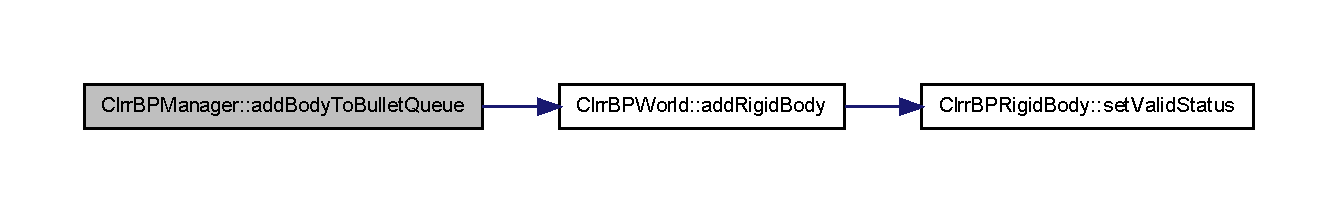
\includegraphics[width=400pt]{class_c_irr_b_p_manager_af5b96f07769449e5b4a7adb8485e027f_cgraph}
\end{center}
\end{figure}


\hypertarget{class_c_irr_b_p_manager_a61ed9d76cfe90285f6e7d80b5870406f}{
\index{CIrrBPManager@{CIrrBPManager}!addRigidBox@{addRigidBox}}
\index{addRigidBox@{addRigidBox}!CIrrBPManager@{CIrrBPManager}}
\subsubsection[{addRigidBox}]{\setlength{\rightskip}{0pt plus 5cm}{\bf CIrrBPBoxBody}$\ast$ CIrrBPManager::addRigidBox (
\begin{DoxyParamCaption}
\item[{ISceneNode $\ast$}]{ node, }
\item[{irr::f32}]{ mass, }
\item[{irr::s32}]{ bodyId = {\ttfamily -\/1}}
\end{DoxyParamCaption}
)}}
\label{class_c_irr_b_p_manager_a61ed9d76cfe90285f6e7d80b5870406f}
Adds a rigid box into the world. 
\begin{DoxyParams}{Parameters}
\item[{\em node}]scene node to which engage the body \item[{\em mass}]body's mass \item[{\em bodyId}]a irrlicht-\/style body id \end{DoxyParams}
\begin{DoxyReturn}{Returns}
Pointer to the object. 
\end{DoxyReturn}
\hypertarget{class_c_irr_b_p_manager_ac351ba81cf28a33bac69bc348860cd48}{
\index{CIrrBPManager@{CIrrBPManager}!addRigidCapsule@{addRigidCapsule}}
\index{addRigidCapsule@{addRigidCapsule}!CIrrBPManager@{CIrrBPManager}}
\subsubsection[{addRigidCapsule}]{\setlength{\rightskip}{0pt plus 5cm}{\bf CIrrBPCapsuleBody}$\ast$ CIrrBPManager::addRigidCapsule (
\begin{DoxyParamCaption}
\item[{ISceneNode $\ast$}]{ node, }
\item[{irr::f32}]{ mass, }
\item[{irr::s32}]{ bodyId = {\ttfamily -\/1}, }
\item[{BODY\_\-OR}]{ bodyOrientationAxis = {\ttfamily AUTO}}
\end{DoxyParamCaption}
)}}
\label{class_c_irr_b_p_manager_ac351ba81cf28a33bac69bc348860cd48}
Adds a rigid capsule into the world 
\begin{DoxyParams}{Parameters}
\item[{\em node}]scene node to which engage the body \item[{\em mass}]body's mass \item[{\em bodyId}]a irrlicht-\/style body id \item[{\em bodyOrientation}]the object' axis orientation. (====) has an X orientation. \end{DoxyParams}
\begin{DoxyReturn}{Returns}
Pointer to the object. 
\end{DoxyReturn}
\hypertarget{class_c_irr_b_p_manager_a810377e264480789138dc4b9ac5145d4}{
\index{CIrrBPManager@{CIrrBPManager}!addRigidCone@{addRigidCone}}
\index{addRigidCone@{addRigidCone}!CIrrBPManager@{CIrrBPManager}}
\subsubsection[{addRigidCone}]{\setlength{\rightskip}{0pt plus 5cm}{\bf CIrrBPConeBody}$\ast$ CIrrBPManager::addRigidCone (
\begin{DoxyParamCaption}
\item[{ISceneNode $\ast$}]{ node, }
\item[{irr::f32}]{ mass, }
\item[{irr::s32}]{ bodyId = {\ttfamily -\/1}, }
\item[{BODY\_\-OR}]{ bodyOrientationAxis = {\ttfamily AUTO}}
\end{DoxyParamCaption}
)}}
\label{class_c_irr_b_p_manager_a810377e264480789138dc4b9ac5145d4}
Adds a rigid cone into the world 
\begin{DoxyParams}{Parameters}
\item[{\em node}]scene node to which engage the body \item[{\em mass}]body's mass \item[{\em bodyId}]a irrlicht-\/style body id \item[{\em bodyOrientation}]the object' axis orientation. /$\backslash$ has an Y orientation. \end{DoxyParams}
\begin{DoxyReturn}{Returns}
Pointer to the object. 
\end{DoxyReturn}
\hypertarget{class_c_irr_b_p_manager_a7866f42ff533e69342c9ad370f07aa23}{
\index{CIrrBPManager@{CIrrBPManager}!addRigidCylinder@{addRigidCylinder}}
\index{addRigidCylinder@{addRigidCylinder}!CIrrBPManager@{CIrrBPManager}}
\subsubsection[{addRigidCylinder}]{\setlength{\rightskip}{0pt plus 5cm}{\bf CIrrBPCylinderBody}$\ast$ CIrrBPManager::addRigidCylinder (
\begin{DoxyParamCaption}
\item[{ISceneNode $\ast$}]{ node, }
\item[{irr::f32}]{ mass, }
\item[{irr::s32}]{ bodyId = {\ttfamily -\/1}, }
\item[{BODY\_\-OR}]{ bodyOrientationAxis = {\ttfamily AUTO}}
\end{DoxyParamCaption}
)}}
\label{class_c_irr_b_p_manager_a7866f42ff533e69342c9ad370f07aa23}
Adds a rigid cylinder into the world 
\begin{DoxyParams}{Parameters}
\item[{\em node}]scene node to which engage the body \item[{\em mass}]body's mass \item[{\em bodyId}]a irrlicht-\/style body id \item[{\em bodyOrientation}]the object' axis orientation. For example \mbox{[}====\mbox{]} has an X orientation. \end{DoxyParams}
\begin{DoxyReturn}{Returns}
Pointer to the object. 
\end{DoxyReturn}
\hypertarget{class_c_irr_b_p_manager_aebbe19de8a748a7c66d5d0efc16dc5eb}{
\index{CIrrBPManager@{CIrrBPManager}!addRigidSphere@{addRigidSphere}}
\index{addRigidSphere@{addRigidSphere}!CIrrBPManager@{CIrrBPManager}}
\subsubsection[{addRigidSphere}]{\setlength{\rightskip}{0pt plus 5cm}{\bf CIrrBPSphereBody}$\ast$ CIrrBPManager::addRigidSphere (
\begin{DoxyParamCaption}
\item[{ISceneNode $\ast$}]{ node, }
\item[{irr::f32}]{ mass, }
\item[{irr::s32}]{ bodyId = {\ttfamily -\/1}}
\end{DoxyParamCaption}
)}}
\label{class_c_irr_b_p_manager_aebbe19de8a748a7c66d5d0efc16dc5eb}
Adds a rigid sphere into the world 
\begin{DoxyParams}{Parameters}
\item[{\em node}]scene node to which engage the body \item[{\em mass}]body's mass \item[{\em bodyId}]a irrlicht-\/style body id \end{DoxyParams}
\begin{DoxyReturn}{Returns}
Pointer to the object. 
\end{DoxyReturn}
\hypertarget{class_c_irr_b_p_manager_a14eef4c19ac93cf7dff82544637833e0}{
\index{CIrrBPManager@{CIrrBPManager}!addTrimesh@{addTrimesh}}
\index{addTrimesh@{addTrimesh}!CIrrBPManager@{CIrrBPManager}}
\subsubsection[{addTrimesh}]{\setlength{\rightskip}{0pt plus 5cm}{\bf CIrrBPTrimesh}$\ast$ CIrrBPManager::addTrimesh (
\begin{DoxyParamCaption}
\item[{IMeshSceneNode $\ast$}]{ node, }
\item[{irr::f32}]{ mass, }
\item[{irr::s32}]{ bodyId = {\ttfamily -\/1}}
\end{DoxyParamCaption}
)}}
\label{class_c_irr_b_p_manager_a14eef4c19ac93cf7dff82544637833e0}
Adds a rigid trimesh into the world 
\begin{DoxyParams}{Parameters}
\item[{\em node}]scene node to which engage the body \item[{\em mass}]body's mass \item[{\em bodyId}]a irrlicht-\/style body id \end{DoxyParams}
\begin{DoxyReturn}{Returns}
Pointer to the object. 
\end{DoxyReturn}
\hypertarget{class_c_irr_b_p_manager_ad565fee43722307839908de9aab70344}{
\index{CIrrBPManager@{CIrrBPManager}!addTrimesh@{addTrimesh}}
\index{addTrimesh@{addTrimesh}!CIrrBPManager@{CIrrBPManager}}
\subsubsection[{addTrimesh}]{\setlength{\rightskip}{0pt plus 5cm}{\bf CIrrBPTrimesh}$\ast$ CIrrBPManager::addTrimesh (
\begin{DoxyParamCaption}
\item[{IAnimatedMeshSceneNode $\ast$}]{ node, }
\item[{irr::f32}]{ mass, }
\item[{irr::s32}]{ bodyId = {\ttfamily -\/1}}
\end{DoxyParamCaption}
)}}
\label{class_c_irr_b_p_manager_ad565fee43722307839908de9aab70344}
Adds a rigid trimesh into the world 
\begin{DoxyParams}{Parameters}
\item[{\em node}]scene node to which engage the body \item[{\em mass}]body's mass \item[{\em bodyId}]a irrlicht-\/style body id \end{DoxyParams}
\begin{DoxyReturn}{Returns}
Pointer to the object. 
\end{DoxyReturn}
\hypertarget{class_c_irr_b_p_manager_ae6c1ebbc11dec61a856bcc7b5c6394ce}{
\index{CIrrBPManager@{CIrrBPManager}!buildConeTwistConstraint@{buildConeTwistConstraint}}
\index{buildConeTwistConstraint@{buildConeTwistConstraint}!CIrrBPManager@{CIrrBPManager}}
\subsubsection[{buildConeTwistConstraint}]{\setlength{\rightskip}{0pt plus 5cm}{\bf CIrrBPConeTwistConstraint} $\ast$ CIrrBPManager::buildConeTwistConstraint (
\begin{DoxyParamCaption}
\item[{{\bf CIrrBPRigidBody} $\ast$}]{ bodyA, }
\item[{{\bf CIrrBPRigidBody} $\ast$}]{ bodyB, }
\item[{const vector3df \&}]{ pivotInA = {\ttfamily vector3df(0,0,0)}, }
\item[{const vector3df \&}]{ pivotInB = {\ttfamily vector3df(0,0,0)}}
\end{DoxyParamCaption}
)}}
\label{class_c_irr_b_p_manager_ae6c1ebbc11dec61a856bcc7b5c6394ce}
Builds a cone twist constraint to the bodies. A cone-\/twist can be used to simulate ragdoll joints (shoulders, legs..)


\begin{DoxyParams}{Parameters}
\item[{\em bodyA}]The first body \item[{\em bodyB}]The second body \item[{\em pivotInA}]The constraint position in A \item[{\em pivotInB}]The constraint position in B \end{DoxyParams}
\begin{DoxyReturn}{Returns}
pointer to the constraint 
\end{DoxyReturn}
\hypertarget{class_c_irr_b_p_manager_a87b2610eaba14775ac81992ff71ab436}{
\index{CIrrBPManager@{CIrrBPManager}!buildHingeConstraint@{buildHingeConstraint}}
\index{buildHingeConstraint@{buildHingeConstraint}!CIrrBPManager@{CIrrBPManager}}
\subsubsection[{buildHingeConstraint}]{\setlength{\rightskip}{0pt plus 5cm}{\bf CIrrBPHingeConstraint} $\ast$ CIrrBPManager::buildHingeConstraint (
\begin{DoxyParamCaption}
\item[{{\bf CIrrBPRigidBody} $\ast$}]{ bodyA, }
\item[{const vector3df \&}]{ pivotInA, }
\item[{const vector3df \&}]{ axisInA}
\end{DoxyParamCaption}
)}}
\label{class_c_irr_b_p_manager_a87b2610eaba14775ac81992ff71ab436}
Builds and attach a hinge constraint to the body.


\begin{DoxyParams}{Parameters}
\item[{\em bodyA}]The first body \item[{\em pivotInA}]The constraint position in A \item[{\em axisInA}]The axis position in A \end{DoxyParams}
\begin{DoxyReturn}{Returns}
pointer to the constraint 
\end{DoxyReturn}
\hypertarget{class_c_irr_b_p_manager_a8a61e921b487d6249e46022b6e9b5ccf}{
\index{CIrrBPManager@{CIrrBPManager}!buildHingeConstraint@{buildHingeConstraint}}
\index{buildHingeConstraint@{buildHingeConstraint}!CIrrBPManager@{CIrrBPManager}}
\subsubsection[{buildHingeConstraint}]{\setlength{\rightskip}{0pt plus 5cm}{\bf CIrrBPHingeConstraint} $\ast$ CIrrBPManager::buildHingeConstraint (
\begin{DoxyParamCaption}
\item[{{\bf CIrrBPRigidBody} $\ast$}]{ bodyA, }
\item[{{\bf CIrrBPRigidBody} $\ast$}]{ bodyB, }
\item[{const vector3df \&}]{ pivotInA, }
\item[{const vector3df \&}]{ pivotInB, }
\item[{const vector3df \&}]{ axisInA, }
\item[{const vector3df \&}]{ axisInB}
\end{DoxyParamCaption}
)}}
\label{class_c_irr_b_p_manager_a8a61e921b487d6249e46022b6e9b5ccf}
Builds and attach a hinge constraint to the body.


\begin{DoxyParams}{Parameters}
\item[{\em bodyA}]The first body \item[{\em bodyB}]The second body \item[{\em pivotInA}]The constraint position in A \item[{\em pivotInB}]The constraint position in B \item[{\em axisInA}]The axis position in A \item[{\em axisInB}]The axis position in B \end{DoxyParams}
\begin{DoxyReturn}{Returns}
pointer to the constraint 
\end{DoxyReturn}
\hypertarget{class_c_irr_b_p_manager_a19a7a9108ded5c076d307efdb390d58a}{
\index{CIrrBPManager@{CIrrBPManager}!buildP2PConstraint@{buildP2PConstraint}}
\index{buildP2PConstraint@{buildP2PConstraint}!CIrrBPManager@{CIrrBPManager}}
\subsubsection[{buildP2PConstraint}]{\setlength{\rightskip}{0pt plus 5cm}{\bf CIrrBPP2PConstraint} $\ast$ CIrrBPManager::buildP2PConstraint (
\begin{DoxyParamCaption}
\item[{{\bf CIrrBPRigidBody} $\ast$}]{ bodyA, }
\item[{const vector3df \&}]{ pivotInA = {\ttfamily vector3df(0,0,0)}}
\end{DoxyParamCaption}
)}}
\label{class_c_irr_b_p_manager_a19a7a9108ded5c076d307efdb390d58a}
Builds and attach a point-\/to-\/point constraint to the body.


\begin{DoxyParams}{Parameters}
\item[{\em bodyA}]The first body \item[{\em pivotInA}]The constraint position in A \end{DoxyParams}
\begin{DoxyReturn}{Returns}
pointer to the constraint 
\end{DoxyReturn}
\hypertarget{class_c_irr_b_p_manager_a1a2dc64a93a8770dfed3ba7f77972c70}{
\index{CIrrBPManager@{CIrrBPManager}!buildP2PConstraint@{buildP2PConstraint}}
\index{buildP2PConstraint@{buildP2PConstraint}!CIrrBPManager@{CIrrBPManager}}
\subsubsection[{buildP2PConstraint}]{\setlength{\rightskip}{0pt plus 5cm}{\bf CIrrBPP2PConstraint} $\ast$ CIrrBPManager::buildP2PConstraint (
\begin{DoxyParamCaption}
\item[{{\bf CIrrBPRigidBody} $\ast$}]{ bodyA, }
\item[{{\bf CIrrBPRigidBody} $\ast$}]{ bodyB, }
\item[{const vector3df \&}]{ pivotInA = {\ttfamily vector3df(0,0,0)}, }
\item[{const vector3df \&}]{ pivotInB = {\ttfamily vector3df(0,0,0)}}
\end{DoxyParamCaption}
)}}
\label{class_c_irr_b_p_manager_a1a2dc64a93a8770dfed3ba7f77972c70}
Builds and attach a point-\/to-\/point constraint to the bodies.


\begin{DoxyParams}{Parameters}
\item[{\em bodyA}]The first body \item[{\em bodyB}]The second body \item[{\em pivotInA}]The constraint position in A \item[{\em pivotInB}]The constraint position in B \end{DoxyParams}
\begin{DoxyReturn}{Returns}
pointer to the constraint 
\end{DoxyReturn}
\hypertarget{class_c_irr_b_p_manager_af916152de29ba8c7c9e727dfe5a1c8af}{
\index{CIrrBPManager@{CIrrBPManager}!buildSlideConstraint@{buildSlideConstraint}}
\index{buildSlideConstraint@{buildSlideConstraint}!CIrrBPManager@{CIrrBPManager}}
\subsubsection[{buildSlideConstraint}]{\setlength{\rightskip}{0pt plus 5cm}{\bf CIrrBPSlideConstraint} $\ast$ CIrrBPManager::buildSlideConstraint (
\begin{DoxyParamCaption}
\item[{{\bf CIrrBPRigidBody} $\ast$}]{ bodyA, }
\item[{{\bf CIrrBPRigidBody} $\ast$}]{ bodyB, }
\item[{const vector3df \&}]{ pivotInA = {\ttfamily vector3df(0,0,0)}, }
\item[{const vector3df \&}]{ pivotInB = {\ttfamily vector3df(0,0,0)}, }
\item[{bool}]{ autoadapt = {\ttfamily true}, }
\item[{bool}]{ rotatepiston = {\ttfamily true}}
\end{DoxyParamCaption}
)}}
\label{class_c_irr_b_p_manager_af916152de29ba8c7c9e727dfe5a1c8af}
Builds and attach a Slide Constraint to the bodies. The last 2 parameters will only works if there is a static object.\par
 Please also note that due to internal conversions, if you place the moving body to a 0.0f position, the object will be moved toward a NEAR 0 value.\par



\begin{DoxyParams}{Parameters}
\item[{\em bodyA}]The first body \item[{\em bodyB}]The second body \item[{\em pivotInA}]The constraint position in A (0,0,0 by default) \item[{\em pivotInB}]The constraint position in B (0,0,0 by default) \item[{\em autoadapt}]If one body is static, and this flag is setted to false. The Slide will be only orthogonal \item[{\em rotatepiston}]If setted to true, the dynamic object (piston) will be rotated in the slide direction. \end{DoxyParams}
\begin{DoxyReturn}{Returns}
pointer to the constraint 
\end{DoxyReturn}
\hypertarget{class_c_irr_b_p_manager_a868af77531e0eb62d14ee060d2c91158}{
\index{CIrrBPManager@{CIrrBPManager}!createCollisionDeleteAnimator@{createCollisionDeleteAnimator}}
\index{createCollisionDeleteAnimator@{createCollisionDeleteAnimator}!CIrrBPManager@{CIrrBPManager}}
\subsubsection[{createCollisionDeleteAnimator}]{\setlength{\rightskip}{0pt plus 5cm}{\bf CIrrBPCollisionDeleteAnimator} $\ast$ CIrrBPManager::createCollisionDeleteAnimator (
\begin{DoxyParamCaption}
\item[{CIB\_\-DFLAG}]{ delFlag}
\end{DoxyParamCaption}
)}}
\label{class_c_irr_b_p_manager_a868af77531e0eb62d14ee060d2c91158}
Creates an on-\/event collision delete animator


\begin{DoxyParams}{Parameters}
\item[{\em delFlag}]The flag that will set the deletion condition \end{DoxyParams}
\begin{DoxyReturn}{Returns}
pointer to the animator 
\end{DoxyReturn}
\hypertarget{class_c_irr_b_p_manager_a34d992b091c917aa9a0febddadf26141}{
\index{CIrrBPManager@{CIrrBPManager}!createDeleteAnimator@{createDeleteAnimator}}
\index{createDeleteAnimator@{createDeleteAnimator}!CIrrBPManager@{CIrrBPManager}}
\subsubsection[{createDeleteAnimator}]{\setlength{\rightskip}{0pt plus 5cm}{\bf CIrrBPDeleteAnimator} $\ast$ CIrrBPManager::createDeleteAnimator (
\begin{DoxyParamCaption}
\item[{irr::u32}]{ timeMs}
\end{DoxyParamCaption}
)}}
\label{class_c_irr_b_p_manager_a34d992b091c917aa9a0febddadf26141}
Creates a delete animator to attach to a body.


\begin{DoxyParams}{Parameters}
\item[{\em timeMs}]Time after which the body will be deleted \end{DoxyParams}
\begin{DoxyReturn}{Returns}
pointer to the animator 
\end{DoxyReturn}
\hypertarget{class_c_irr_b_p_manager_ab82cddba1a3acd79119e2708680acffb}{
\index{CIrrBPManager@{CIrrBPManager}!drop@{drop}}
\index{drop@{drop}!CIrrBPManager@{CIrrBPManager}}
\subsubsection[{drop}]{\setlength{\rightskip}{0pt plus 5cm}void CIrrBPManager::drop (
\begin{DoxyParamCaption}
{}
\end{DoxyParamCaption}
)\hspace{0.3cm}{\ttfamily  \mbox{[}inline\mbox{]}}}}
\label{class_c_irr_b_p_manager_ab82cddba1a3acd79119e2708680acffb}
Drops the bullet manager \hypertarget{class_c_irr_b_p_manager_ad48556f70ceddf1501ccc11120ef511c}{
\index{CIrrBPManager@{CIrrBPManager}!getRigidBodyFromId@{getRigidBodyFromId}}
\index{getRigidBodyFromId@{getRigidBodyFromId}!CIrrBPManager@{CIrrBPManager}}
\subsubsection[{getRigidBodyFromId}]{\setlength{\rightskip}{0pt plus 5cm}{\bf CIrrBPRigidBody}$\ast$ CIrrBPManager::getRigidBodyFromId (
\begin{DoxyParamCaption}
\item[{irr::s32}]{ id}
\end{DoxyParamCaption}
)\hspace{0.3cm}{\ttfamily  \mbox{[}inline\mbox{]}}}}
\label{class_c_irr_b_p_manager_ad48556f70ceddf1501ccc11120ef511c}
Gets a rigid Body from a id. 
\begin{DoxyParams}{Parameters}
\item[{\em id}]The id to search for \end{DoxyParams}
\begin{DoxyReturn}{Returns}
Pointer to the first rigid body with this id. Returns NULL if no bodies couldn't be found. 
\end{DoxyReturn}
\hypertarget{class_c_irr_b_p_manager_a6da3e324ed8e5eb8332588de2fdde1a0}{
\index{CIrrBPManager@{CIrrBPManager}!getRigidBodyFromName@{getRigidBodyFromName}}
\index{getRigidBodyFromName@{getRigidBodyFromName}!CIrrBPManager@{CIrrBPManager}}
\subsubsection[{getRigidBodyFromName}]{\setlength{\rightskip}{0pt plus 5cm}{\bf CIrrBPRigidBody}$\ast$ CIrrBPManager::getRigidBodyFromName (
\begin{DoxyParamCaption}
\item[{irr::c8 $\ast$}]{ name}
\end{DoxyParamCaption}
)\hspace{0.3cm}{\ttfamily  \mbox{[}inline\mbox{]}}}}
\label{class_c_irr_b_p_manager_a6da3e324ed8e5eb8332588de2fdde1a0}
Gets a rigid Body from a name. 
\begin{DoxyParams}{Parameters}
\item[{\em name}]The name to search for \end{DoxyParams}
\begin{DoxyReturn}{Returns}
Pointer to the first rigid body with this name. Returns NULL if no bodies couldn't be found. 
\end{DoxyReturn}
\hypertarget{class_c_irr_b_p_manager_a6dda0b5ecda7508c5b44e29fe72a6d27}{
\index{CIrrBPManager@{CIrrBPManager}!getRigidBodyFromUId@{getRigidBodyFromUId}}
\index{getRigidBodyFromUId@{getRigidBodyFromUId}!CIrrBPManager@{CIrrBPManager}}
\subsubsection[{getRigidBodyFromUId}]{\setlength{\rightskip}{0pt plus 5cm}{\bf CIrrBPRigidBody}$\ast$ CIrrBPManager::getRigidBodyFromUId (
\begin{DoxyParamCaption}
\item[{irr::u32}]{ uid}
\end{DoxyParamCaption}
)\hspace{0.3cm}{\ttfamily  \mbox{[}inline\mbox{]}}}}
\label{class_c_irr_b_p_manager_a6dda0b5ecda7508c5b44e29fe72a6d27}
Gets a rigid Body from a unique id. 
\begin{DoxyParams}{Parameters}
\item[{\em id}]The unique id to search for \end{DoxyParams}
\begin{DoxyReturn}{Returns}
Pointer to the first rigid body with this id. Returns NULL if no bodies couldn't be found. 
\end{DoxyReturn}
\hypertarget{class_c_irr_b_p_manager_acdfaf5f8c351d72c4d9680cb75372ae3}{
\index{CIrrBPManager@{CIrrBPManager}!getWorld@{getWorld}}
\index{getWorld@{getWorld}!CIrrBPManager@{CIrrBPManager}}
\subsubsection[{getWorld}]{\setlength{\rightskip}{0pt plus 5cm}{\bf CIrrBPWorld}$\ast$ CIrrBPManager::getWorld (
\begin{DoxyParamCaption}
{}
\end{DoxyParamCaption}
)\hspace{0.3cm}{\ttfamily  \mbox{[}inline\mbox{]}}}}
\label{class_c_irr_b_p_manager_acdfaf5f8c351d72c4d9680cb75372ae3}
Gets the world pointer. \begin{DoxyReturn}{Returns}
Pointer to the world object 
\end{DoxyReturn}
\hypertarget{class_c_irr_b_p_manager_ad4896d9448a572add3c84ca5118c6baa}{
\index{CIrrBPManager@{CIrrBPManager}!removeBody@{removeBody}}
\index{removeBody@{removeBody}!CIrrBPManager@{CIrrBPManager}}
\subsubsection[{removeBody}]{\setlength{\rightskip}{0pt plus 5cm}void CIrrBPManager::removeBody (
\begin{DoxyParamCaption}
\item[{{\bf CIrrBPRigidBody} $\ast$}]{ body}
\end{DoxyParamCaption}
)}}
\label{class_c_irr_b_p_manager_ad4896d9448a572add3c84ca5118c6baa}
Removes a body from the bullet queue. Call this function instead of using body's internal drop function 

Here is the call graph for this function:\nopagebreak
\begin{figure}[H]
\begin{center}
\leavevmode
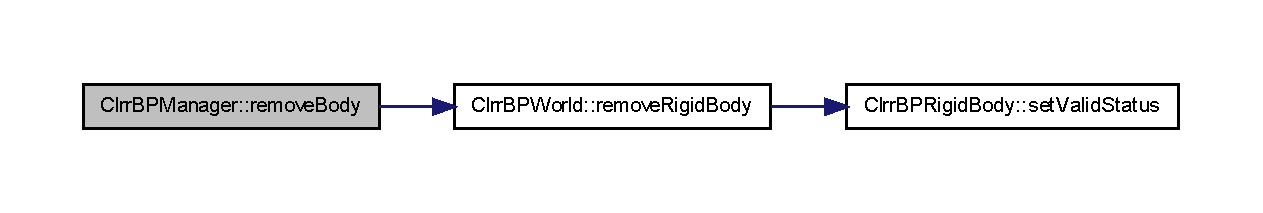
\includegraphics[width=400pt]{class_c_irr_b_p_manager_ad4896d9448a572add3c84ca5118c6baa_cgraph}
\end{center}
\end{figure}


\hypertarget{class_c_irr_b_p_manager_ad3eea990a27f0ce4cfc2564c475f55f2}{
\index{CIrrBPManager@{CIrrBPManager}!setWorldGravity@{setWorldGravity}}
\index{setWorldGravity@{setWorldGravity}!CIrrBPManager@{CIrrBPManager}}
\subsubsection[{setWorldGravity}]{\setlength{\rightskip}{0pt plus 5cm}void CIrrBPManager::setWorldGravity (
\begin{DoxyParamCaption}
\item[{const vector3df \&}]{ Gravity}
\end{DoxyParamCaption}
)\hspace{0.3cm}{\ttfamily  \mbox{[}inline\mbox{]}}}}
\label{class_c_irr_b_p_manager_ad3eea990a27f0ce4cfc2564c475f55f2}
Sets the gravity in the world. 
\begin{DoxyParams}{Parameters}
\item[{\em Gravity}]vector containing direction \end{DoxyParams}
\hypertarget{class_c_irr_b_p_manager_ae058cbb1d7ed8c4c3813a7205c7f2d9d}{
\index{CIrrBPManager@{CIrrBPManager}!stepSimulation@{stepSimulation}}
\index{stepSimulation@{stepSimulation}!CIrrBPManager@{CIrrBPManager}}
\subsubsection[{stepSimulation}]{\setlength{\rightskip}{0pt plus 5cm}REALINLINE void CIrrBPManager::stepSimulation (
\begin{DoxyParamCaption}
{}
\end{DoxyParamCaption}
)\hspace{0.3cm}{\ttfamily  \mbox{[}inline\mbox{]}}}}
\label{class_c_irr_b_p_manager_ae058cbb1d7ed8c4c3813a7205c7f2d9d}
Steps the simulation. It must be called each frame loop to step the bullet' simulation. 

The documentation for this class was generated from the following files:\begin{DoxyCompactItemize}
\item 
E:/Documenti/Lavori Stefano/ProgettoFPS/Engine/Engine/IrrBP/include/CIrrBPManager.h\item 
E:/Documenti/Lavori Stefano/ProgettoFPS/Engine/Engine/IrrBP/src/CIrrBPManager.cpp\end{DoxyCompactItemize}

\hypertarget{class_c_irr_b_p_p2_p_constraint}{
\section{CIrrBPP2PConstraint Class Reference}
\label{class_c_irr_b_p_p2_p_constraint}\index{CIrrBPP2PConstraint@{CIrrBPP2PConstraint}}
}


Inherits \hyperlink{class_c_irr_b_p_constraint}{CIrrBPConstraint}.



Collaboration diagram for CIrrBPP2PConstraint:\nopagebreak
\begin{figure}[H]
\begin{center}
\leavevmode
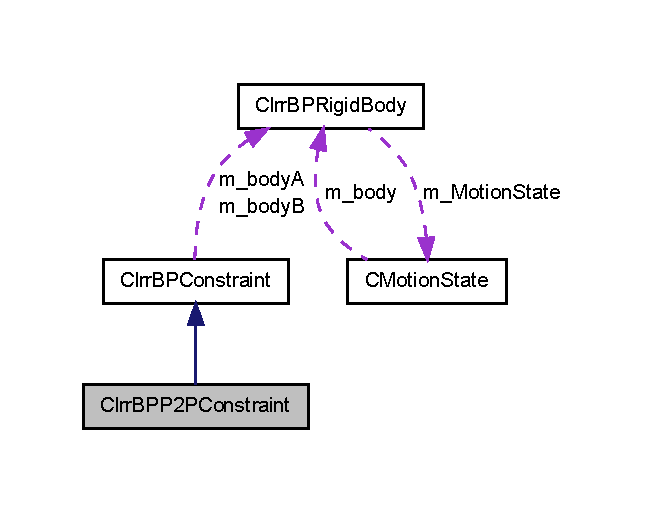
\includegraphics[width=310pt]{class_c_irr_b_p_p2_p_constraint__coll__graph}
\end{center}
\end{figure}
\subsection*{Public Member Functions}
\begin{DoxyCompactItemize}
\item 
\hypertarget{class_c_irr_b_p_p2_p_constraint_a7bcd4e6890eda89a126d139db2691bbc}{
{\bfseries CIrrBPP2PConstraint} (\hyperlink{class_c_irr_b_p_rigid_body}{CIrrBPRigidBody} $\ast$bodyA, const vector3df \&pivotInA)}
\label{class_c_irr_b_p_p2_p_constraint_a7bcd4e6890eda89a126d139db2691bbc}

\item 
\hypertarget{class_c_irr_b_p_p2_p_constraint_a0fcb7e338114b3bd920d370e2cef017b}{
{\bfseries CIrrBPP2PConstraint} (\hyperlink{class_c_irr_b_p_rigid_body}{CIrrBPRigidBody} $\ast$bodyA, \hyperlink{class_c_irr_b_p_rigid_body}{CIrrBPRigidBody} $\ast$bodyB, const vector3df \&pivotInA, const vector3df \&pivotInB)}
\label{class_c_irr_b_p_p2_p_constraint_a0fcb7e338114b3bd920d370e2cef017b}

\item 
void \hyperlink{class_c_irr_b_p_p2_p_constraint_abc3ec07fbc260cb8f88727fd8e9fc2c6}{drop} ()
\end{DoxyCompactItemize}


\subsection{Member Function Documentation}
\hypertarget{class_c_irr_b_p_p2_p_constraint_abc3ec07fbc260cb8f88727fd8e9fc2c6}{
\index{CIrrBPP2PConstraint@{CIrrBPP2PConstraint}!drop@{drop}}
\index{drop@{drop}!CIrrBPP2PConstraint@{CIrrBPP2PConstraint}}
\subsubsection[{drop}]{\setlength{\rightskip}{0pt plus 5cm}void CIrrBPP2PConstraint::drop (
\begin{DoxyParamCaption}
{}
\end{DoxyParamCaption}
)\hspace{0.3cm}{\ttfamily  \mbox{[}inline, virtual\mbox{]}}}}
\label{class_c_irr_b_p_p2_p_constraint_abc3ec07fbc260cb8f88727fd8e9fc2c6}
Drop Function. This function should not be used. The destructor will be called automatically by the World Object. 

Implements \hyperlink{class_c_irr_b_p_constraint_a2718ef7118d60646a5cfa2dfe5a44795}{CIrrBPConstraint}.



The documentation for this class was generated from the following files:\begin{DoxyCompactItemize}
\item 
E:/Documenti/Lavori Stefano/ProgettoFPS/Engine/Engine/IrrBP/include/constraint/CIrrBPP2PConstraint.h\item 
E:/Documenti/Lavori Stefano/ProgettoFPS/Engine/Engine/IrrBP/src/constraint/CIrrBPP2PConstraint.cpp\end{DoxyCompactItemize}

\hypertarget{class_c_irr_b_p_rigid_body}{
\section{CIrrBPRigidBody Class Reference}
\label{class_c_irr_b_p_rigid_body}\index{CIrrBPRigidBody@{CIrrBPRigidBody}}
}


Inherits \hyperlink{class_c_irr_b_p_collision_object}{CIrrBPCollisionObject}.



Inherited by \hyperlink{class_c_irr_b_p_box_body}{CIrrBPBoxBody}, \hyperlink{class_c_irr_b_p_capsule_body}{CIrrBPCapsuleBody}, \hyperlink{class_c_irr_b_p_cone_body}{CIrrBPConeBody}, \hyperlink{class_c_irr_b_p_cylinder_body}{CIrrBPCylinderBody}, \hyperlink{class_c_irr_b_p_sphere_body}{CIrrBPSphereBody}, and \hyperlink{class_c_irr_b_p_trimesh}{CIrrBPTrimesh}.



Collaboration diagram for CIrrBPRigidBody:\nopagebreak
\begin{figure}[H]
\begin{center}
\leavevmode
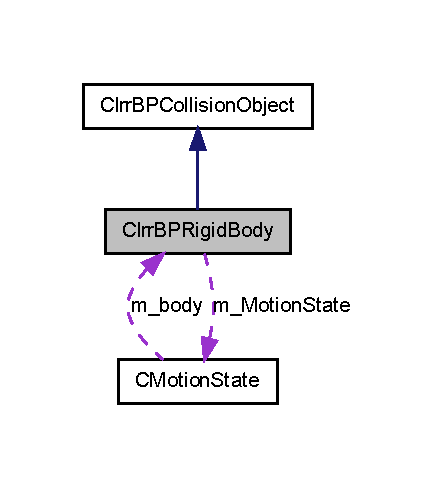
\includegraphics[width=209pt]{class_c_irr_b_p_rigid_body__coll__graph}
\end{center}
\end{figure}
\subsection*{Public Member Functions}
\begin{DoxyCompactItemize}
\item 
virtual void \hyperlink{class_c_irr_b_p_rigid_body_a961d442e36e78260e7a6f203fd0c11e9}{drop} ()=0
\item 
\hypertarget{class_c_irr_b_p_rigid_body_a93948bb4c79cea0b3172c5fe1146007c}{
virtual void {\bfseries applyTorque} (const vector3df \&torque)}
\label{class_c_irr_b_p_rigid_body_a93948bb4c79cea0b3172c5fe1146007c}

\item 
\hypertarget{class_c_irr_b_p_rigid_body_aa3fbb7492486b64b0f53e3243f20d3db}{
virtual void {\bfseries applyForce} (const vector3df \&force, const vector3df \&rel\_\-pos)}
\label{class_c_irr_b_p_rigid_body_aa3fbb7492486b64b0f53e3243f20d3db}

\item 
\hypertarget{class_c_irr_b_p_rigid_body_a4697f05241c551fbd80d2786507ceed4}{
virtual void {\bfseries applyCentralImpulse} (const vector3df \&impulse)}
\label{class_c_irr_b_p_rigid_body_a4697f05241c551fbd80d2786507ceed4}

\item 
\hypertarget{class_c_irr_b_p_rigid_body_aea6add503a694f1b54f9b406217416d1}{
virtual void {\bfseries applyCentralForce} (const vector3df \&force)}
\label{class_c_irr_b_p_rigid_body_aea6add503a694f1b54f9b406217416d1}

\item 
\hypertarget{class_c_irr_b_p_rigid_body_a633f6f306f2b061870c78ae5137fe238}{
virtual void {\bfseries applyTorqueImpulse} (const vector3df \&torque)}
\label{class_c_irr_b_p_rigid_body_a633f6f306f2b061870c78ae5137fe238}

\item 
\hypertarget{class_c_irr_b_p_rigid_body_a7cda3cfa35a7b6325b67bc48cc1adcdb}{
virtual void {\bfseries applyImpulse} (const vector3df \&impulse, const vector3df \&rel\_\-pos)}
\label{class_c_irr_b_p_rigid_body_a7cda3cfa35a7b6325b67bc48cc1adcdb}

\item 
\hypertarget{class_c_irr_b_p_rigid_body_a3e4f7b3000b5955bd8731be4104d963a}{
virtual btRigidBody $\ast$ {\bfseries getBodyPtr} ()}
\label{class_c_irr_b_p_rigid_body_a3e4f7b3000b5955bd8731be4104d963a}

\item 
\hypertarget{class_c_irr_b_p_rigid_body_a1242a37feff707d535c66508afc4bc7f}{
virtual \hyperlink{class_c_motion_state}{CMotionState} $\ast$ {\bfseries getMotionState} ()}
\label{class_c_irr_b_p_rigid_body_a1242a37feff707d535c66508afc4bc7f}

\item 
\hypertarget{class_c_irr_b_p_rigid_body_ad0db19bf9575c316e235eb669d499084}{
virtual bool {\bfseries isStaticObject} ()}
\label{class_c_irr_b_p_rigid_body_ad0db19bf9575c316e235eb669d499084}

\item 
\hypertarget{class_c_irr_b_p_rigid_body_ac15067d38996295fbe1ea274ec8d245f}{
virtual ISceneNode $\ast$ {\bfseries getIrrlichtNode} ()}
\label{class_c_irr_b_p_rigid_body_ac15067d38996295fbe1ea274ec8d245f}

\end{DoxyCompactItemize}
\subsection*{Protected Attributes}
\begin{DoxyCompactItemize}
\item 
\hypertarget{class_c_irr_b_p_rigid_body_aa49da88d7c108171dadf441915cd2d1c}{
ISceneNode $\ast$ {\bfseries m\_\-IrrSceneNode}}
\label{class_c_irr_b_p_rigid_body_aa49da88d7c108171dadf441915cd2d1c}

\item 
\hypertarget{class_c_irr_b_p_rigid_body_a913c50a2e04215904c69351a000ad5b4}{
\hyperlink{class_c_motion_state}{CMotionState} $\ast$ {\bfseries m\_\-MotionState}}
\label{class_c_irr_b_p_rigid_body_a913c50a2e04215904c69351a000ad5b4}

\item 
\hypertarget{class_c_irr_b_p_rigid_body_a21e96ec352898c0342b2155edb6334b5}{
btCollisionShape $\ast$ {\bfseries m\_\-Shape}}
\label{class_c_irr_b_p_rigid_body_a21e96ec352898c0342b2155edb6334b5}

\item 
\hypertarget{class_c_irr_b_p_rigid_body_a97f19d79af040a5c7a7ace9ae8c5880d}{
btRigidBody $\ast$ {\bfseries m\_\-RigidBody}}
\label{class_c_irr_b_p_rigid_body_a97f19d79af040a5c7a7ace9ae8c5880d}

\end{DoxyCompactItemize}


\subsection{Member Function Documentation}
\hypertarget{class_c_irr_b_p_rigid_body_a961d442e36e78260e7a6f203fd0c11e9}{
\index{CIrrBPRigidBody@{CIrrBPRigidBody}!drop@{drop}}
\index{drop@{drop}!CIrrBPRigidBody@{CIrrBPRigidBody}}
\subsubsection[{drop}]{\setlength{\rightskip}{0pt plus 5cm}virtual void CIrrBPRigidBody::drop (
\begin{DoxyParamCaption}
{}
\end{DoxyParamCaption}
)\hspace{0.3cm}{\ttfamily  \mbox{[}pure virtual\mbox{]}}}}
\label{class_c_irr_b_p_rigid_body_a961d442e36e78260e7a6f203fd0c11e9}
Drop Function. This function should not be used. The destructor will be called automatically by the World Object. 

Implements \hyperlink{class_c_irr_b_p_collision_object_a8fda1f4f6c5f34f42c51645baeb436ca}{CIrrBPCollisionObject}.



Implemented in \hyperlink{class_c_irr_b_p_box_body_a144a57bdaaa418c5851f0beb97bdc44b}{CIrrBPBoxBody}, \hyperlink{class_c_irr_b_p_capsule_body_ab9815977583c6135b4b42dee8f536098}{CIrrBPCapsuleBody}, \hyperlink{class_c_irr_b_p_cone_body_a47470fa549f852a5d315f0decb4d195a}{CIrrBPConeBody}, \hyperlink{class_c_irr_b_p_cylinder_body_a966bec7330f778f276294601fc7e0c45}{CIrrBPCylinderBody}, \hyperlink{class_c_irr_b_p_sphere_body_ae5060da603f81cb391c320ef35ae80eb}{CIrrBPSphereBody}, and \hyperlink{class_c_irr_b_p_trimesh_a5106e0daefa0a7dd6198311390711255}{CIrrBPTrimesh}.



The documentation for this class was generated from the following files:\begin{DoxyCompactItemize}
\item 
E:/Documenti/Lavori Stefano/ProgettoFPS/Engine/Engine/IrrBP/include/body/CIrrBPRigidBody.h\item 
E:/Documenti/Lavori Stefano/ProgettoFPS/Engine/Engine/IrrBP/src/body/CIrrBPRigidBody.cpp\end{DoxyCompactItemize}

\hypertarget{class_c_irr_b_p_slide_constraint}{
\section{CIrrBPSlideConstraint Class Reference}
\label{class_c_irr_b_p_slide_constraint}\index{CIrrBPSlideConstraint@{CIrrBPSlideConstraint}}
}


Inherits \hyperlink{class_c_irr_b_p_constraint}{CIrrBPConstraint}.



Collaboration diagram for CIrrBPSlideConstraint:\nopagebreak
\begin{figure}[H]
\begin{center}
\leavevmode
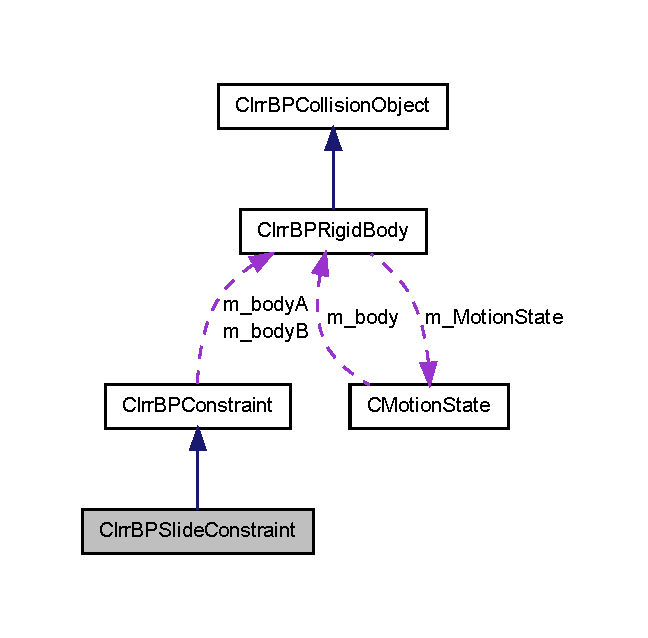
\includegraphics[width=311pt]{class_c_irr_b_p_slide_constraint__coll__graph}
\end{center}
\end{figure}
\subsection*{Public Member Functions}
\begin{DoxyCompactItemize}
\item 
\hyperlink{class_c_irr_b_p_slide_constraint_a4912466dafa0ed9f93907498b2bd3866}{CIrrBPSlideConstraint} (\hyperlink{class_c_irr_b_p_rigid_body}{CIrrBPRigidBody} $\ast$bodyA, \hyperlink{class_c_irr_b_p_rigid_body}{CIrrBPRigidBody} $\ast$bodyB, const vector3df \&pivotInA=vector3df(0, 0, 0), const vector3df \&pivotInB=vector3df(0, 0, 0), bool autoadapt=true, bool rotatepiston=true)
\item 
\hypertarget{class_c_irr_b_p_slide_constraint_a8af14b26091df650f28ff8f2d53e372f}{
irr::f32 {\bfseries getLowerLinLimit} ()}
\label{class_c_irr_b_p_slide_constraint_a8af14b26091df650f28ff8f2d53e372f}

\item 
\hypertarget{class_c_irr_b_p_slide_constraint_aa0d2b6ed2de89734bf91613c5dac90cb}{
void {\bfseries setLowerLinLimit} (irr::f32 lowerLimit)}
\label{class_c_irr_b_p_slide_constraint_aa0d2b6ed2de89734bf91613c5dac90cb}

\item 
\hypertarget{class_c_irr_b_p_slide_constraint_adbfda3683804e88ab93581017f4e565c}{
irr::f32 {\bfseries getUpperLinLimit} ()}
\label{class_c_irr_b_p_slide_constraint_adbfda3683804e88ab93581017f4e565c}

\item 
\hypertarget{class_c_irr_b_p_slide_constraint_a49fea36c98c957f91feb695053d730fb}{
void {\bfseries setUpperLinLimit} (irr::f32 upperLimit)}
\label{class_c_irr_b_p_slide_constraint_a49fea36c98c957f91feb695053d730fb}

\item 
\hypertarget{class_c_irr_b_p_slide_constraint_afc55508bd7ebdf3ae2ef3fe8493b21cd}{
irr::f32 {\bfseries getLowerAngLimit} ()}
\label{class_c_irr_b_p_slide_constraint_afc55508bd7ebdf3ae2ef3fe8493b21cd}

\item 
\hypertarget{class_c_irr_b_p_slide_constraint_a52210fc1232fc9b0bdbc2c4189d3f637}{
void {\bfseries setLowerAngLimit} (irr::f32 lowerLimit)}
\label{class_c_irr_b_p_slide_constraint_a52210fc1232fc9b0bdbc2c4189d3f637}

\item 
\hypertarget{class_c_irr_b_p_slide_constraint_a161828edc475d822945e386b41236511}{
irr::f32 {\bfseries getUpperAngLimit} ()}
\label{class_c_irr_b_p_slide_constraint_a161828edc475d822945e386b41236511}

\item 
\hypertarget{class_c_irr_b_p_slide_constraint_a5d12930f4f88460c8c29aa2cbd1f2576}{
void {\bfseries setUpperAngLimit} (irr::f32 upperLimit)}
\label{class_c_irr_b_p_slide_constraint_a5d12930f4f88460c8c29aa2cbd1f2576}

\item 
\hypertarget{class_c_irr_b_p_slide_constraint_ad1b9a262ecd02b45964af15c90102964}{
irr::f32 {\bfseries getSoftnessDirLin} ()}
\label{class_c_irr_b_p_slide_constraint_ad1b9a262ecd02b45964af15c90102964}

\item 
\hypertarget{class_c_irr_b_p_slide_constraint_af77d5604440529036eb6082cb64a1dca}{
irr::f32 {\bfseries getRestitutionDirLin} ()}
\label{class_c_irr_b_p_slide_constraint_af77d5604440529036eb6082cb64a1dca}

\item 
\hypertarget{class_c_irr_b_p_slide_constraint_abc5f21289b1aa30ec82bdf9f3da3bced}{
irr::f32 {\bfseries getDampingDirLin} ()}
\label{class_c_irr_b_p_slide_constraint_abc5f21289b1aa30ec82bdf9f3da3bced}

\item 
\hypertarget{class_c_irr_b_p_slide_constraint_ab699aa633c9a792d21d7ffc70b5e55b5}{
irr::f32 {\bfseries getSoftnessDirAng} ()}
\label{class_c_irr_b_p_slide_constraint_ab699aa633c9a792d21d7ffc70b5e55b5}

\item 
\hypertarget{class_c_irr_b_p_slide_constraint_a89f5b7cbcd24d2840f8c87f579b80cbb}{
irr::f32 {\bfseries getRestitutionDirAng} ()}
\label{class_c_irr_b_p_slide_constraint_a89f5b7cbcd24d2840f8c87f579b80cbb}

\item 
\hypertarget{class_c_irr_b_p_slide_constraint_ade91f0cac4cc594bea029b5b85b114d0}{
irr::f32 {\bfseries getDampingDirAng} ()}
\label{class_c_irr_b_p_slide_constraint_ade91f0cac4cc594bea029b5b85b114d0}

\item 
\hypertarget{class_c_irr_b_p_slide_constraint_a679bd66d7abc97908f2309b4648287b9}{
irr::f32 {\bfseries getSoftnessLimLin} ()}
\label{class_c_irr_b_p_slide_constraint_a679bd66d7abc97908f2309b4648287b9}

\item 
\hypertarget{class_c_irr_b_p_slide_constraint_a1c57bb2a3bd265b4ef31c5d84c58fb85}{
irr::f32 {\bfseries getRestitutionLimLin} ()}
\label{class_c_irr_b_p_slide_constraint_a1c57bb2a3bd265b4ef31c5d84c58fb85}

\item 
\hypertarget{class_c_irr_b_p_slide_constraint_a0671729442e18d9c1c8a518a665a0f47}{
irr::f32 {\bfseries getDampingLimLin} ()}
\label{class_c_irr_b_p_slide_constraint_a0671729442e18d9c1c8a518a665a0f47}

\item 
\hypertarget{class_c_irr_b_p_slide_constraint_a2727ec43c4a047aa4a57c14e788bf985}{
irr::f32 {\bfseries getSoftnessLimAng} ()}
\label{class_c_irr_b_p_slide_constraint_a2727ec43c4a047aa4a57c14e788bf985}

\item 
\hypertarget{class_c_irr_b_p_slide_constraint_a1b75677266d386f16ca1be43b37bd4c9}{
irr::f32 {\bfseries getRestitutionLimAng} ()}
\label{class_c_irr_b_p_slide_constraint_a1b75677266d386f16ca1be43b37bd4c9}

\item 
\hypertarget{class_c_irr_b_p_slide_constraint_a88ba4d72523a5ff2ed4fb0c9014e1978}{
irr::f32 {\bfseries getDampingLimAng} ()}
\label{class_c_irr_b_p_slide_constraint_a88ba4d72523a5ff2ed4fb0c9014e1978}

\item 
\hypertarget{class_c_irr_b_p_slide_constraint_a1ff0ec2d56187fa983a7dd6f98bcb4f5}{
irr::f32 {\bfseries getSoftnessOrthoLin} ()}
\label{class_c_irr_b_p_slide_constraint_a1ff0ec2d56187fa983a7dd6f98bcb4f5}

\item 
\hypertarget{class_c_irr_b_p_slide_constraint_a169a38d61ef500efc0077b177cc5dc77}{
irr::f32 {\bfseries getRestitutionOrthoLin} ()}
\label{class_c_irr_b_p_slide_constraint_a169a38d61ef500efc0077b177cc5dc77}

\item 
\hypertarget{class_c_irr_b_p_slide_constraint_aab7c26e8d1951d261e4cbafeba1a272c}{
irr::f32 {\bfseries getDampingOrthoLin} ()}
\label{class_c_irr_b_p_slide_constraint_aab7c26e8d1951d261e4cbafeba1a272c}

\item 
\hypertarget{class_c_irr_b_p_slide_constraint_a80534a95b8f07b198b13a08ae75d329a}{
irr::f32 {\bfseries getSoftnessOrthoAng} ()}
\label{class_c_irr_b_p_slide_constraint_a80534a95b8f07b198b13a08ae75d329a}

\item 
\hypertarget{class_c_irr_b_p_slide_constraint_ae03fa1278ce572062d46cd13e33b708f}{
irr::f32 {\bfseries getRestitutionOrthoAng} ()}
\label{class_c_irr_b_p_slide_constraint_ae03fa1278ce572062d46cd13e33b708f}

\item 
\hypertarget{class_c_irr_b_p_slide_constraint_af31506ff537543dd817023f8f4599cc1}{
irr::f32 {\bfseries getDampingOrthoAng} ()}
\label{class_c_irr_b_p_slide_constraint_af31506ff537543dd817023f8f4599cc1}

\item 
\hypertarget{class_c_irr_b_p_slide_constraint_a397b97506df91156da00c37a26cc53c8}{
void {\bfseries setSoftnessDirLin} (irr::f32 softnessDirLin)}
\label{class_c_irr_b_p_slide_constraint_a397b97506df91156da00c37a26cc53c8}

\item 
\hypertarget{class_c_irr_b_p_slide_constraint_a32a9fcfd4ab74ffc80a06a36fe303678}{
void {\bfseries setRestitutionDirLin} (irr::f32 restitutionDirLin)}
\label{class_c_irr_b_p_slide_constraint_a32a9fcfd4ab74ffc80a06a36fe303678}

\item 
\hypertarget{class_c_irr_b_p_slide_constraint_a398722b0643a49337be23b5a2ca1aa89}{
void {\bfseries setDampingDirLin} (irr::f32 dampingDirLin)}
\label{class_c_irr_b_p_slide_constraint_a398722b0643a49337be23b5a2ca1aa89}

\item 
\hypertarget{class_c_irr_b_p_slide_constraint_a129735643ca5e0c355304b2ed967db74}{
void {\bfseries setSoftnessDirAng} (irr::f32 softnessDirAng)}
\label{class_c_irr_b_p_slide_constraint_a129735643ca5e0c355304b2ed967db74}

\item 
\hypertarget{class_c_irr_b_p_slide_constraint_aa427ff6f1bca3651a291e2564db83598}{
void {\bfseries setRestitutionDirAng} (irr::f32 restitutionDirAng)}
\label{class_c_irr_b_p_slide_constraint_aa427ff6f1bca3651a291e2564db83598}

\item 
\hypertarget{class_c_irr_b_p_slide_constraint_ab38bb01e738213517eed482668c66b19}{
void {\bfseries setDampingDirAng} (irr::f32 dampingDirAng)}
\label{class_c_irr_b_p_slide_constraint_ab38bb01e738213517eed482668c66b19}

\item 
\hypertarget{class_c_irr_b_p_slide_constraint_a220dbde37eeb940ec072b342a3605eb0}{
void {\bfseries setSoftnessLimLin} (irr::f32 softnessLimLin)}
\label{class_c_irr_b_p_slide_constraint_a220dbde37eeb940ec072b342a3605eb0}

\item 
\hypertarget{class_c_irr_b_p_slide_constraint_aa65843d056d31700196bc6da695b8f2c}{
void {\bfseries setRestitutionLimLin} (irr::f32 restitutionLimLin)}
\label{class_c_irr_b_p_slide_constraint_aa65843d056d31700196bc6da695b8f2c}

\item 
\hypertarget{class_c_irr_b_p_slide_constraint_a97a82079ab5fa785bd412f93f40927b5}{
void {\bfseries setDampingLimLin} (irr::f32 dampingLimLin)}
\label{class_c_irr_b_p_slide_constraint_a97a82079ab5fa785bd412f93f40927b5}

\item 
\hypertarget{class_c_irr_b_p_slide_constraint_a63e2aa99061d8121218c8b304628d8f7}{
void {\bfseries setSoftnessLimAng} (irr::f32 softnessLimAng)}
\label{class_c_irr_b_p_slide_constraint_a63e2aa99061d8121218c8b304628d8f7}

\item 
\hypertarget{class_c_irr_b_p_slide_constraint_acea0e8abfa4295e95dd148b3a02a11e7}{
void {\bfseries setRestitutionLimAng} (irr::f32 restitutionLimAng)}
\label{class_c_irr_b_p_slide_constraint_acea0e8abfa4295e95dd148b3a02a11e7}

\item 
\hypertarget{class_c_irr_b_p_slide_constraint_ae83561e6ecbf6f3f19628de4b13b42e0}{
void {\bfseries setDampingLimAng} (irr::f32 dampingLimAng)}
\label{class_c_irr_b_p_slide_constraint_ae83561e6ecbf6f3f19628de4b13b42e0}

\item 
\hypertarget{class_c_irr_b_p_slide_constraint_a3c52720f6bbfd8a419b3e316cf176839}{
void {\bfseries setSoftnessOrthoLin} (irr::f32 softnessOrthoLin)}
\label{class_c_irr_b_p_slide_constraint_a3c52720f6bbfd8a419b3e316cf176839}

\item 
\hypertarget{class_c_irr_b_p_slide_constraint_a26f84b0323c7107bb99ebdc4ce1193fd}{
void {\bfseries setRestitutionOrthoLin} (irr::f32 restitutionOrthoLin)}
\label{class_c_irr_b_p_slide_constraint_a26f84b0323c7107bb99ebdc4ce1193fd}

\item 
\hypertarget{class_c_irr_b_p_slide_constraint_a9f7c4cc5ab4076e0539575d4c66bf384}{
void {\bfseries setDampingOrthoLin} (irr::f32 dampingOrthoLin)}
\label{class_c_irr_b_p_slide_constraint_a9f7c4cc5ab4076e0539575d4c66bf384}

\item 
\hypertarget{class_c_irr_b_p_slide_constraint_a1847f06bc037af050a887e9c139e0681}{
void {\bfseries setSoftnessOrthoAng} (irr::f32 softnessOrthoAng)}
\label{class_c_irr_b_p_slide_constraint_a1847f06bc037af050a887e9c139e0681}

\item 
\hypertarget{class_c_irr_b_p_slide_constraint_ae244cad578807d16899cfc4e1b92a3df}{
void {\bfseries setRestitutionOrthoAng} (irr::f32 restitutionOrthoAng)}
\label{class_c_irr_b_p_slide_constraint_ae244cad578807d16899cfc4e1b92a3df}

\item 
\hypertarget{class_c_irr_b_p_slide_constraint_a1390d767b6988d6158053c3a5f2b839f}{
void {\bfseries setDampingOrthoAng} (irr::f32 dampingOrthoAng)}
\label{class_c_irr_b_p_slide_constraint_a1390d767b6988d6158053c3a5f2b839f}

\item 
\hypertarget{class_c_irr_b_p_slide_constraint_a3565a2a2cd586e2dc248db1d5c595a05}{
void {\bfseries setPoweredLinMotor} (bool onOff)}
\label{class_c_irr_b_p_slide_constraint_a3565a2a2cd586e2dc248db1d5c595a05}

\item 
\hypertarget{class_c_irr_b_p_slide_constraint_aab1330eb896120c51334eb617154982e}{
bool {\bfseries getPoweredLinMotor} ()}
\label{class_c_irr_b_p_slide_constraint_aab1330eb896120c51334eb617154982e}

\item 
void \hyperlink{class_c_irr_b_p_slide_constraint_acaaf3cfaba14b8c126ab548f7c21c2b6}{drop} ()
\end{DoxyCompactItemize}
\subsection*{Protected Attributes}
\begin{DoxyCompactItemize}
\item 
\hypertarget{class_c_irr_b_p_slide_constraint_addc70a99abc01da40b54ccb18bc35ab5}{
btSliderConstraint $\ast$ {\bfseries m\_\-fixedConstraint}}
\label{class_c_irr_b_p_slide_constraint_addc70a99abc01da40b54ccb18bc35ab5}

\end{DoxyCompactItemize}


\subsection{Constructor \& Destructor Documentation}
\hypertarget{class_c_irr_b_p_slide_constraint_a4912466dafa0ed9f93907498b2bd3866}{
\index{CIrrBPSlideConstraint@{CIrrBPSlideConstraint}!CIrrBPSlideConstraint@{CIrrBPSlideConstraint}}
\index{CIrrBPSlideConstraint@{CIrrBPSlideConstraint}!CIrrBPSlideConstraint@{CIrrBPSlideConstraint}}
\subsubsection[{CIrrBPSlideConstraint}]{\setlength{\rightskip}{0pt plus 5cm}CIrrBPSlideConstraint::CIrrBPSlideConstraint (
\begin{DoxyParamCaption}
\item[{{\bf CIrrBPRigidBody} $\ast$}]{ bodyA, }
\item[{{\bf CIrrBPRigidBody} $\ast$}]{ bodyB, }
\item[{const vector3df \&}]{ pivotInA = {\ttfamily vector3df(0,0,0)}, }
\item[{const vector3df \&}]{ pivotInB = {\ttfamily vector3df(0,0,0)}, }
\item[{bool}]{ autoadapt = {\ttfamily true}, }
\item[{bool}]{ rotatepiston = {\ttfamily true}}
\end{DoxyParamCaption}
)}}
\label{class_c_irr_b_p_slide_constraint_a4912466dafa0ed9f93907498b2bd3866}
Constructor.\par
 The last 2 parameters will only works if there is a static object.\par
 Please also note that due to internal conversions, if you place the moving body to a 0.0f position, the object will be moved toward a NEAR 0 value.\par



\begin{DoxyParams}{Parameters}
\item[{\em bodyA}]The first body \item[{\em bodyB}]The second body \item[{\em pivotInA}]The constraint position in A (0,0,0 by default) \item[{\em pivotInB}]The constraint position in B (0,0,0 by default) \item[{\em autoadapt}]If one body is static, and this flag is setted to false. The Slide will be only orthogonal \item[{\em rotatepiston}]If setted to true, the dynamic object (piston) will be rotated in the slide direction. \end{DoxyParams}


\subsection{Member Function Documentation}
\hypertarget{class_c_irr_b_p_slide_constraint_acaaf3cfaba14b8c126ab548f7c21c2b6}{
\index{CIrrBPSlideConstraint@{CIrrBPSlideConstraint}!drop@{drop}}
\index{drop@{drop}!CIrrBPSlideConstraint@{CIrrBPSlideConstraint}}
\subsubsection[{drop}]{\setlength{\rightskip}{0pt plus 5cm}void CIrrBPSlideConstraint::drop (
\begin{DoxyParamCaption}
{}
\end{DoxyParamCaption}
)\hspace{0.3cm}{\ttfamily  \mbox{[}inline, virtual\mbox{]}}}}
\label{class_c_irr_b_p_slide_constraint_acaaf3cfaba14b8c126ab548f7c21c2b6}
Drop Function. This function should not be used. The destructor will be called automatically by the World Object. 

Implements \hyperlink{class_c_irr_b_p_constraint_a2718ef7118d60646a5cfa2dfe5a44795}{CIrrBPConstraint}.



The documentation for this class was generated from the following files:\begin{DoxyCompactItemize}
\item 
E:/Documenti/Lavori Stefano/ProgettoFPS/Engine/Engine/IrrBP/include/constraint/CIrrBPSlideConstraint.h\item 
E:/Documenti/Lavori Stefano/ProgettoFPS/Engine/Engine/IrrBP/src/constraint/CIrrBPSlideConstraint.cpp\end{DoxyCompactItemize}

\hypertarget{class_c_irr_b_p_sphere_body}{
\section{CIrrBPSphereBody Class Reference}
\label{class_c_irr_b_p_sphere_body}\index{CIrrBPSphereBody@{CIrrBPSphereBody}}
}


Inherits \hyperlink{class_c_irr_b_p_rigid_body}{CIrrBPRigidBody}.



Collaboration diagram for CIrrBPSphereBody:\nopagebreak
\begin{figure}[H]
\begin{center}
\leavevmode
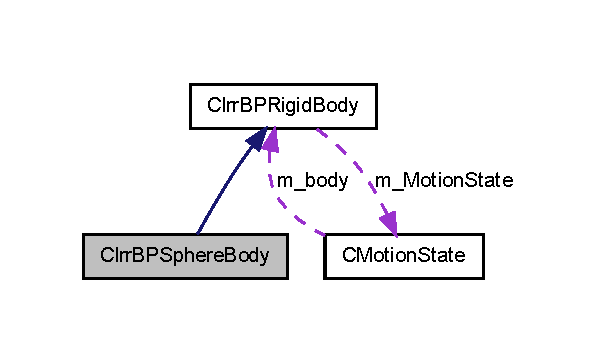
\includegraphics[width=287pt]{class_c_irr_b_p_sphere_body__coll__graph}
\end{center}
\end{figure}
\subsection*{Public Member Functions}
\begin{DoxyCompactItemize}
\item 
virtual void \hyperlink{class_c_irr_b_p_sphere_body_ae5060da603f81cb391c320ef35ae80eb}{drop} ()
\item 
\hypertarget{class_c_irr_b_p_sphere_body_afb99648bc34a2a8a1ae997078251d2d1}{
{\bfseries CIrrBPSphereBody} (ISceneNode $\ast$node, irr::f32 mass, irr::s32 bodyId=-\/1)}
\label{class_c_irr_b_p_sphere_body_afb99648bc34a2a8a1ae997078251d2d1}

\end{DoxyCompactItemize}


\subsection{Member Function Documentation}
\hypertarget{class_c_irr_b_p_sphere_body_ae5060da603f81cb391c320ef35ae80eb}{
\index{CIrrBPSphereBody@{CIrrBPSphereBody}!drop@{drop}}
\index{drop@{drop}!CIrrBPSphereBody@{CIrrBPSphereBody}}
\subsubsection[{drop}]{\setlength{\rightskip}{0pt plus 5cm}virtual void CIrrBPSphereBody::drop (
\begin{DoxyParamCaption}
{}
\end{DoxyParamCaption}
)\hspace{0.3cm}{\ttfamily  \mbox{[}inline, virtual\mbox{]}}}}
\label{class_c_irr_b_p_sphere_body_ae5060da603f81cb391c320ef35ae80eb}
Drop Function. This function should not be used. The destructor will be called automatically by the World Object. 

Implements \hyperlink{class_c_irr_b_p_rigid_body_a961d442e36e78260e7a6f203fd0c11e9}{CIrrBPRigidBody}.



The documentation for this class was generated from the following files:\begin{DoxyCompactItemize}
\item 
E:/Documenti/Lavori Stefano/ProgettoFPS/Engine/Engine/IrrBP/include/body/CIrrBPSphereBody.h\item 
E:/Documenti/Lavori Stefano/ProgettoFPS/Engine/Engine/IrrBP/src/body/CIrrBPSphereBody.cpp\end{DoxyCompactItemize}

\hypertarget{class_c_irr_b_p_trimesh}{
\section{CIrrBPTrimesh Class Reference}
\label{class_c_irr_b_p_trimesh}\index{CIrrBPTrimesh@{CIrrBPTrimesh}}
}


Inherits \hyperlink{class_c_irr_b_p_rigid_body}{CIrrBPRigidBody}.



Collaboration diagram for CIrrBPTrimesh:\nopagebreak
\begin{figure}[H]
\begin{center}
\leavevmode
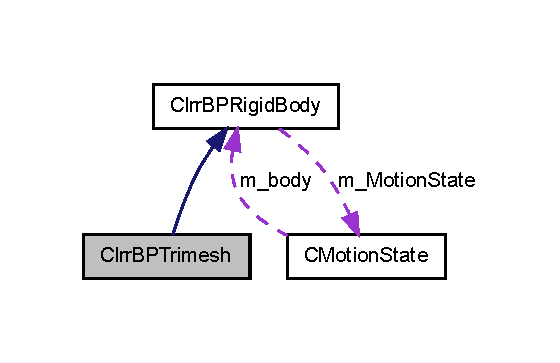
\includegraphics[width=269pt]{class_c_irr_b_p_trimesh__coll__graph}
\end{center}
\end{figure}
\subsection*{Public Member Functions}
\begin{DoxyCompactItemize}
\item 
virtual void \hyperlink{class_c_irr_b_p_trimesh_a5106e0daefa0a7dd6198311390711255}{drop} ()
\item 
\hypertarget{class_c_irr_b_p_trimesh_adcc11a8bcf9461ff7cc44092bbe56c09}{
{\bfseries CIrrBPTrimesh} (IAnimatedMeshSceneNode $\ast$node, irr::f32 mass, irr::s32 bodyId=-\/1)}
\label{class_c_irr_b_p_trimesh_adcc11a8bcf9461ff7cc44092bbe56c09}

\item 
\hypertarget{class_c_irr_b_p_trimesh_a8f8683ddff5e11df3c40b746a14cf193}{
{\bfseries CIrrBPTrimesh} (IMeshSceneNode $\ast$node, irr::f32 mass, irr::s32 bodyId=-\/1)}
\label{class_c_irr_b_p_trimesh_a8f8683ddff5e11df3c40b746a14cf193}

\end{DoxyCompactItemize}


\subsection{Member Function Documentation}
\hypertarget{class_c_irr_b_p_trimesh_a5106e0daefa0a7dd6198311390711255}{
\index{CIrrBPTrimesh@{CIrrBPTrimesh}!drop@{drop}}
\index{drop@{drop}!CIrrBPTrimesh@{CIrrBPTrimesh}}
\subsubsection[{drop}]{\setlength{\rightskip}{0pt plus 5cm}virtual void CIrrBPTrimesh::drop (
\begin{DoxyParamCaption}
{}
\end{DoxyParamCaption}
)\hspace{0.3cm}{\ttfamily  \mbox{[}inline, virtual\mbox{]}}}}
\label{class_c_irr_b_p_trimesh_a5106e0daefa0a7dd6198311390711255}
Drop Function. This function should not be used. The destructor will be called automatically by the World Object. 

Implements \hyperlink{class_c_irr_b_p_rigid_body_a961d442e36e78260e7a6f203fd0c11e9}{CIrrBPRigidBody}.



The documentation for this class was generated from the following files:\begin{DoxyCompactItemize}
\item 
E:/Documenti/Lavori Stefano/ProgettoFPS/Engine/Engine/IrrBP/include/body/CIrrBPTrimeshBody.h\item 
E:/Documenti/Lavori Stefano/ProgettoFPS/Engine/Engine/IrrBP/src/body/CIrrBPTrimeshBody.cpp\end{DoxyCompactItemize}

\hypertarget{class_c_irr_b_p_world}{
\section{CIrrBPWorld Class Reference}
\label{class_c_irr_b_p_world}\index{CIrrBPWorld@{CIrrBPWorld}}
}
\subsection*{Public Member Functions}
\begin{DoxyCompactItemize}
\item 
\hyperlink{class_c_irr_b_p_world_a585d92e41db74a19bf1cb982ddc0cddc}{CIrrBPWorld} (IrrlichtDevice $\ast$device, const vector3df \&Gravity)
\item 
void \hyperlink{class_c_irr_b_p_world_aa676e88466f927af2ac0c4c8cd94e0f3}{stepSimulation} ()
\item 
irr::u32 \hyperlink{class_c_irr_b_p_world_a0bf527c522426b50d959ab5adc27be4c}{addRigidBody} (\hyperlink{class_c_irr_b_p_rigid_body}{CIrrBPRigidBody} $\ast$body)
\item 
\hypertarget{class_c_irr_b_p_world_a7565f787e92f3c3cf76da072fe175b11}{
void {\bfseries addRigidBodyConstraint} (\hyperlink{class_c_irr_b_p_constraint}{CIrrBPConstraint} $\ast$constraint)}
\label{class_c_irr_b_p_world_a7565f787e92f3c3cf76da072fe175b11}

\item 
void \hyperlink{class_c_irr_b_p_world_a7133c6b9763ac425ac579cdfbda8788b}{removeRigidBody} (\hyperlink{class_c_irr_b_p_rigid_body}{CIrrBPRigidBody} $\ast$body)
\item 
irr::u32 \hyperlink{class_c_irr_b_p_world_a66e4c4aeef5d3ae6f907753860b8fd5a}{getActiveBodies} ()
\item 
\hyperlink{class_c_irr_b_p_rigid_body}{CIrrBPRigidBody} $\ast$ \hyperlink{class_c_irr_b_p_world_a7ebeb8e75b825a493daa1cea6d07aa21}{getRigidBodyFromId} (irr::s32 id)
\item 
\hyperlink{class_c_irr_b_p_rigid_body}{CIrrBPRigidBody} $\ast$ \hyperlink{class_c_irr_b_p_world_a1b96effdaad31a6e05185f2b683a0445}{getRigidBodyFromUId} (irr::u32 uid)
\item 
\hyperlink{class_c_irr_b_p_rigid_body}{CIrrBPRigidBody} $\ast$ \hyperlink{class_c_irr_b_p_world_a1ed94585fa44f0ab99cfa4a1fdc29fcd}{getRigidBodyFromName} (irr::c8 $\ast$name)
\item 
bool \hyperlink{class_c_irr_b_p_world_abc8fc2e0dbc203106e91cb1e944c496a}{isBodyColliding} (\hyperlink{class_c_irr_b_p_rigid_body}{CIrrBPRigidBody} $\ast$body, irr::s32 collMask=-\/1)
\item 
void \hyperlink{class_c_irr_b_p_world_a7cd82f40cde955cb54c1fc0268691be6}{drop} ()
\item 
\hypertarget{class_c_irr_b_p_world_a96e06a9d2b64d474bfd5325d2ffe809e}{
void {\bfseries setGravity} (const vector3df \&newGravity)}
\label{class_c_irr_b_p_world_a96e06a9d2b64d474bfd5325d2ffe809e}

\item 
btDiscreteDynamicsWorld $\ast$ \hyperlink{class_c_irr_b_p_world_aa9b3e5a74f8ee1185247bc58ec6aec0c}{getBulletWorldPtr} ()
\end{DoxyCompactItemize}
\subsection*{Public Attributes}
\begin{DoxyCompactItemize}
\item 
bool \hyperlink{class_c_irr_b_p_world_a4659a995f7b084057cad44480cd09cca}{isClosing}
\end{DoxyCompactItemize}


\subsection{Constructor \& Destructor Documentation}
\hypertarget{class_c_irr_b_p_world_a585d92e41db74a19bf1cb982ddc0cddc}{
\index{CIrrBPWorld@{CIrrBPWorld}!CIrrBPWorld@{CIrrBPWorld}}
\index{CIrrBPWorld@{CIrrBPWorld}!CIrrBPWorld@{CIrrBPWorld}}
\subsubsection[{CIrrBPWorld}]{\setlength{\rightskip}{0pt plus 5cm}CIrrBPWorld::CIrrBPWorld (
\begin{DoxyParamCaption}
\item[{IrrlichtDevice $\ast$}]{ device, }
\item[{const vector3df \&}]{ Gravity}
\end{DoxyParamCaption}
)}}
\label{class_c_irr_b_p_world_a585d92e41db74a19bf1cb982ddc0cddc}
Constructor. 
\begin{DoxyParams}{Parameters}
\item[{\em device}]A pointer to a Irrlicht's device \item[{\em Gravity}]World's Gravity . \end{DoxyParams}


\subsection{Member Function Documentation}
\hypertarget{class_c_irr_b_p_world_a0bf527c522426b50d959ab5adc27be4c}{
\index{CIrrBPWorld@{CIrrBPWorld}!addRigidBody@{addRigidBody}}
\index{addRigidBody@{addRigidBody}!CIrrBPWorld@{CIrrBPWorld}}
\subsubsection[{addRigidBody}]{\setlength{\rightskip}{0pt plus 5cm}irr::u32 CIrrBPWorld::addRigidBody (
\begin{DoxyParamCaption}
\item[{{\bf CIrrBPRigidBody} $\ast$}]{ body}
\end{DoxyParamCaption}
)}}
\label{class_c_irr_b_p_world_a0bf527c522426b50d959ab5adc27be4c}
Adds a rigid Body to the world. 
\begin{DoxyParams}{Parameters}
\item[{\em body}]A pointer to the body that needs to be added \end{DoxyParams}


Here is the call graph for this function:\nopagebreak
\begin{figure}[H]
\begin{center}
\leavevmode
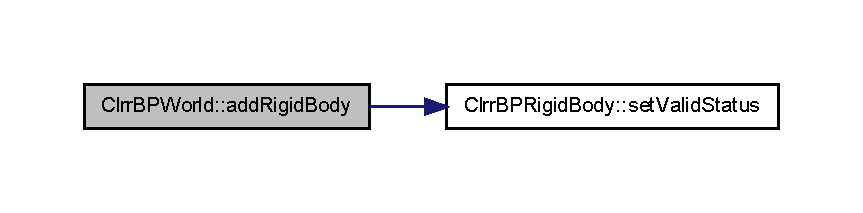
\includegraphics[width=400pt]{class_c_irr_b_p_world_a0bf527c522426b50d959ab5adc27be4c_cgraph}
\end{center}
\end{figure}




Here is the caller graph for this function:\nopagebreak
\begin{figure}[H]
\begin{center}
\leavevmode
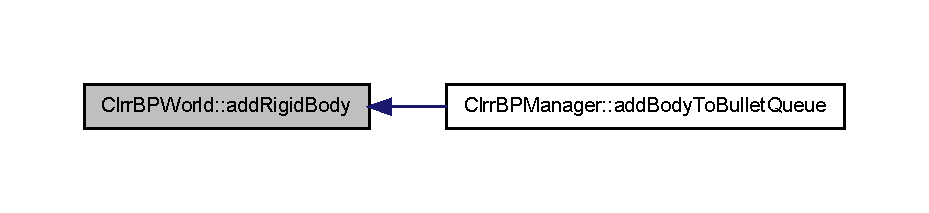
\includegraphics[width=400pt]{class_c_irr_b_p_world_a0bf527c522426b50d959ab5adc27be4c_icgraph}
\end{center}
\end{figure}


\hypertarget{class_c_irr_b_p_world_a7cd82f40cde955cb54c1fc0268691be6}{
\index{CIrrBPWorld@{CIrrBPWorld}!drop@{drop}}
\index{drop@{drop}!CIrrBPWorld@{CIrrBPWorld}}
\subsubsection[{drop}]{\setlength{\rightskip}{0pt plus 5cm}void CIrrBPWorld::drop (
\begin{DoxyParamCaption}
{}
\end{DoxyParamCaption}
)\hspace{0.3cm}{\ttfamily  \mbox{[}inline\mbox{]}}}}
\label{class_c_irr_b_p_world_a7cd82f40cde955cb54c1fc0268691be6}
Drop the world pointer and all his child. Please note that all registered rigid bodies pointers, will be destroyed. \hypertarget{class_c_irr_b_p_world_a66e4c4aeef5d3ae6f907753860b8fd5a}{
\index{CIrrBPWorld@{CIrrBPWorld}!getActiveBodies@{getActiveBodies}}
\index{getActiveBodies@{getActiveBodies}!CIrrBPWorld@{CIrrBPWorld}}
\subsubsection[{getActiveBodies}]{\setlength{\rightskip}{0pt plus 5cm}irr::u32 CIrrBPWorld::getActiveBodies (
\begin{DoxyParamCaption}
{}
\end{DoxyParamCaption}
)\hspace{0.3cm}{\ttfamily  \mbox{[}inline\mbox{]}}}}
\label{class_c_irr_b_p_world_a66e4c4aeef5d3ae6f907753860b8fd5a}
Gets the number of active bodies in the world \begin{DoxyReturn}{Returns}
number of active bodies 
\end{DoxyReturn}
\hypertarget{class_c_irr_b_p_world_aa9b3e5a74f8ee1185247bc58ec6aec0c}{
\index{CIrrBPWorld@{CIrrBPWorld}!getBulletWorldPtr@{getBulletWorldPtr}}
\index{getBulletWorldPtr@{getBulletWorldPtr}!CIrrBPWorld@{CIrrBPWorld}}
\subsubsection[{getBulletWorldPtr}]{\setlength{\rightskip}{0pt plus 5cm}btDiscreteDynamicsWorld$\ast$ CIrrBPWorld::getBulletWorldPtr (
\begin{DoxyParamCaption}
{}
\end{DoxyParamCaption}
)\hspace{0.3cm}{\ttfamily  \mbox{[}inline\mbox{]}}}}
\label{class_c_irr_b_p_world_aa9b3e5a74f8ee1185247bc58ec6aec0c}
Only for internal or expert use. \begin{DoxyReturn}{Returns}
a pointer to the bullet' world object 
\end{DoxyReturn}
\hypertarget{class_c_irr_b_p_world_a7ebeb8e75b825a493daa1cea6d07aa21}{
\index{CIrrBPWorld@{CIrrBPWorld}!getRigidBodyFromId@{getRigidBodyFromId}}
\index{getRigidBodyFromId@{getRigidBodyFromId}!CIrrBPWorld@{CIrrBPWorld}}
\subsubsection[{getRigidBodyFromId}]{\setlength{\rightskip}{0pt plus 5cm}{\bf CIrrBPRigidBody} $\ast$ CIrrBPWorld::getRigidBodyFromId (
\begin{DoxyParamCaption}
\item[{irr::s32}]{ id}
\end{DoxyParamCaption}
)}}
\label{class_c_irr_b_p_world_a7ebeb8e75b825a493daa1cea6d07aa21}
Gets a rigid Body from a id. 
\begin{DoxyParams}{Parameters}
\item[{\em id}]The id to search for \end{DoxyParams}
\begin{DoxyReturn}{Returns}
Pointer to the first rigid body with this id. Returns NULL if no bodies couldn't be found. 
\end{DoxyReturn}
\hypertarget{class_c_irr_b_p_world_a1ed94585fa44f0ab99cfa4a1fdc29fcd}{
\index{CIrrBPWorld@{CIrrBPWorld}!getRigidBodyFromName@{getRigidBodyFromName}}
\index{getRigidBodyFromName@{getRigidBodyFromName}!CIrrBPWorld@{CIrrBPWorld}}
\subsubsection[{getRigidBodyFromName}]{\setlength{\rightskip}{0pt plus 5cm}{\bf CIrrBPRigidBody} $\ast$ CIrrBPWorld::getRigidBodyFromName (
\begin{DoxyParamCaption}
\item[{irr::c8 $\ast$}]{ name}
\end{DoxyParamCaption}
)}}
\label{class_c_irr_b_p_world_a1ed94585fa44f0ab99cfa4a1fdc29fcd}
Gets a rigid Body from a name. 
\begin{DoxyParams}{Parameters}
\item[{\em name}]The name to search for \end{DoxyParams}
\begin{DoxyReturn}{Returns}
Pointer to the first rigid body with this name. Returns NULL if no bodies couldn't be found. 
\end{DoxyReturn}
\hypertarget{class_c_irr_b_p_world_a1b96effdaad31a6e05185f2b683a0445}{
\index{CIrrBPWorld@{CIrrBPWorld}!getRigidBodyFromUId@{getRigidBodyFromUId}}
\index{getRigidBodyFromUId@{getRigidBodyFromUId}!CIrrBPWorld@{CIrrBPWorld}}
\subsubsection[{getRigidBodyFromUId}]{\setlength{\rightskip}{0pt plus 5cm}{\bf CIrrBPRigidBody} $\ast$ CIrrBPWorld::getRigidBodyFromUId (
\begin{DoxyParamCaption}
\item[{irr::u32}]{ uid}
\end{DoxyParamCaption}
)}}
\label{class_c_irr_b_p_world_a1b96effdaad31a6e05185f2b683a0445}
Gets a rigid Body from a unique id. 
\begin{DoxyParams}{Parameters}
\item[{\em id}]The unique id to search for \end{DoxyParams}
\begin{DoxyReturn}{Returns}
Pointer to the first rigid body with this id. Returns NULL if no bodies couldn't be found. 
\end{DoxyReturn}
\hypertarget{class_c_irr_b_p_world_abc8fc2e0dbc203106e91cb1e944c496a}{
\index{CIrrBPWorld@{CIrrBPWorld}!isBodyColliding@{isBodyColliding}}
\index{isBodyColliding@{isBodyColliding}!CIrrBPWorld@{CIrrBPWorld}}
\subsubsection[{isBodyColliding}]{\setlength{\rightskip}{0pt plus 5cm}bool CIrrBPWorld::isBodyColliding (
\begin{DoxyParamCaption}
\item[{{\bf CIrrBPRigidBody} $\ast$}]{ body, }
\item[{irr::s32}]{ collMask = {\ttfamily -\/1}}
\end{DoxyParamCaption}
)}}
\label{class_c_irr_b_p_world_abc8fc2e0dbc203106e91cb1e944c496a}
Verifies if a body is colliding or not. 
\begin{DoxyParams}{Parameters}
\item[{\em body}]body to verify \item[{\em collMask}]not yet full implemented. \end{DoxyParams}
\begin{DoxyReturn}{Returns}
body colliding status. 
\end{DoxyReturn}
\hypertarget{class_c_irr_b_p_world_a7133c6b9763ac425ac579cdfbda8788b}{
\index{CIrrBPWorld@{CIrrBPWorld}!removeRigidBody@{removeRigidBody}}
\index{removeRigidBody@{removeRigidBody}!CIrrBPWorld@{CIrrBPWorld}}
\subsubsection[{removeRigidBody}]{\setlength{\rightskip}{0pt plus 5cm}void CIrrBPWorld::removeRigidBody (
\begin{DoxyParamCaption}
\item[{{\bf CIrrBPRigidBody} $\ast$}]{ body}
\end{DoxyParamCaption}
)}}
\label{class_c_irr_b_p_world_a7133c6b9763ac425ac579cdfbda8788b}
Removes a rigid Body from the world. Please note that the body's Scene Node won't be dropped. 
\begin{DoxyParams}{Parameters}
\item[{\em body}]A pointer to the body that needs to be deleted. \end{DoxyParams}


Here is the call graph for this function:\nopagebreak
\begin{figure}[H]
\begin{center}
\leavevmode
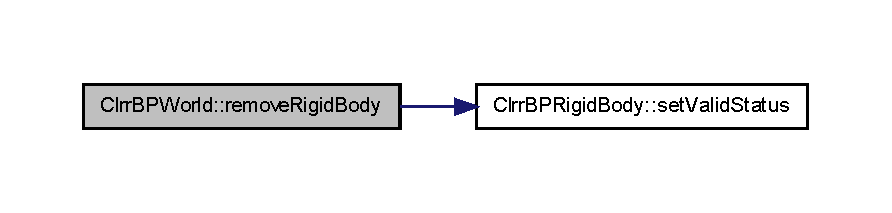
\includegraphics[width=400pt]{class_c_irr_b_p_world_a7133c6b9763ac425ac579cdfbda8788b_cgraph}
\end{center}
\end{figure}




Here is the caller graph for this function:\nopagebreak
\begin{figure}[H]
\begin{center}
\leavevmode
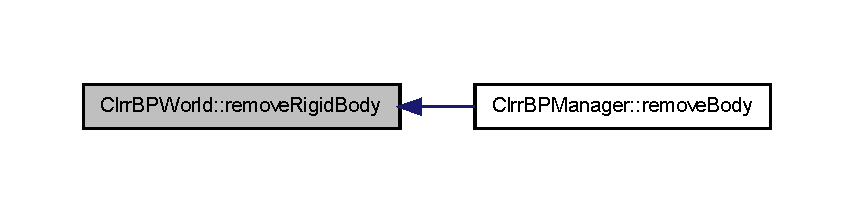
\includegraphics[width=400pt]{class_c_irr_b_p_world_a7133c6b9763ac425ac579cdfbda8788b_icgraph}
\end{center}
\end{figure}


\hypertarget{class_c_irr_b_p_world_aa676e88466f927af2ac0c4c8cd94e0f3}{
\index{CIrrBPWorld@{CIrrBPWorld}!stepSimulation@{stepSimulation}}
\index{stepSimulation@{stepSimulation}!CIrrBPWorld@{CIrrBPWorld}}
\subsubsection[{stepSimulation}]{\setlength{\rightskip}{0pt plus 5cm}void CIrrBPWorld::stepSimulation (
\begin{DoxyParamCaption}
{}
\end{DoxyParamCaption}
)}}
\label{class_c_irr_b_p_world_aa676e88466f927af2ac0c4c8cd94e0f3}
Steps the simulation. It must be called each frame loop to step the bullet' simulation. 

\subsection{Member Data Documentation}
\hypertarget{class_c_irr_b_p_world_a4659a995f7b084057cad44480cd09cca}{
\index{CIrrBPWorld@{CIrrBPWorld}!isClosing@{isClosing}}
\index{isClosing@{isClosing}!CIrrBPWorld@{CIrrBPWorld}}
\subsubsection[{isClosing}]{\setlength{\rightskip}{0pt plus 5cm}bool {\bf CIrrBPWorld::isClosing}}}
\label{class_c_irr_b_p_world_a4659a995f7b084057cad44480cd09cca}
true if world is going to close 

The documentation for this class was generated from the following files:\begin{DoxyCompactItemize}
\item 
E:/Documenti/Lavori Stefano/ProgettoFPS/Engine/Engine/IrrBP/include/CIrrBPWorld.h\item 
E:/Documenti/Lavori Stefano/ProgettoFPS/Engine/Engine/IrrBP/src/CIrrBPWorld.cpp\end{DoxyCompactItemize}

\hypertarget{class_c_motion_state}{
\section{CMotionState Class Reference}
\label{class_c_motion_state}\index{CMotionState@{CMotionState}}
}


Should not be used. Only for internal use.  




{\ttfamily \#include $<$CMotionState.h$>$}



Collaboration diagram for CMotionState:\nopagebreak
\begin{figure}[H]
\begin{center}
\leavevmode
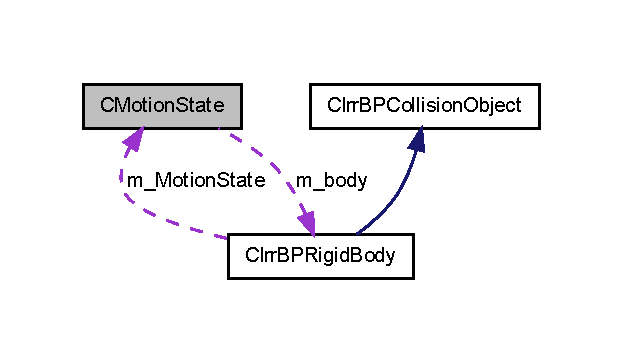
\includegraphics[width=189pt]{class_c_motion_state__coll__graph}
\end{center}
\end{figure}
\subsection*{Public Member Functions}
\begin{DoxyCompactItemize}
\item 
\hypertarget{class_c_motion_state_a0352d243092a662ad672cf5621040adf}{
{\bfseries CMotionState} (\hyperlink{class_c_irr_b_p_rigid_body}{CIrrBPRigidBody} $\ast$body, const btTransform \&startTrans=btTransform::getIdentity(), const btTransform \&centerOfMassOffset=btTransform::getIdentity())}
\label{class_c_motion_state_a0352d243092a662ad672cf5621040adf}

\item 
\hypertarget{class_c_motion_state_a25a63325dc9bd847440d0fc83af77ee6}{
virtual void {\bfseries setWorldTransform} (const btTransform \&worldTrans)}
\label{class_c_motion_state_a25a63325dc9bd847440d0fc83af77ee6}

\end{DoxyCompactItemize}
\subsection*{Protected Attributes}
\begin{DoxyCompactItemize}
\item 
\hypertarget{class_c_motion_state_aff461c9f16ad28d27ae2062029514558}{
\hyperlink{class_c_irr_b_p_rigid_body}{CIrrBPRigidBody} $\ast$ {\bfseries m\_\-body}}
\label{class_c_motion_state_aff461c9f16ad28d27ae2062029514558}

\item 
\hypertarget{class_c_motion_state_a010b74f2e84fccdd4f82c2def2c7529d}{
ISceneNode $\ast$ {\bfseries m\_\-irrNode}}
\label{class_c_motion_state_a010b74f2e84fccdd4f82c2def2c7529d}

\end{DoxyCompactItemize}


\subsection{Detailed Description}
Should not be used. Only for internal use. 

The documentation for this class was generated from the following files:\begin{DoxyCompactItemize}
\item 
E:/Documenti/Lavori Stefano/ProgettoFPS/Engine/Engine/IrrBP/include/CMotionState.h\item 
E:/Documenti/Lavori Stefano/ProgettoFPS/Engine/Engine/IrrBP/src/CMotionState.cpp\end{DoxyCompactItemize}

\printindex
\end{document}
